\subsection{DEFINITION OF A LIE GROUP}

Let \(G\) be a set. A group structure and an analytic K-manifold structure on \(G\) are called compatible if the following condition holds:

(GL) The mapping \((g, h) \mapsto gh^{-1}\) of \(\mathbf{G} \times \mathbf{G}\) into \(\mathbf{G}\) is analytic.

DEFINITION 1. A Lie group over K is a set G with a group structure and an analytic K-manifold structure such that these two structures are compatible.

A Lie group over \(\mathbf{R}\) (resp. \(\mathbf{C},\mathbf{Q}_p\) ) is called a real (resp. complex, \(p\) -adic) Lie group.

Let \(\mathbf{G}\) be a group with an analytic manifold structure. For \(g, h, g_0, h_0\) in \(\mathbf{G}\) ,

\[
g h ^ {- 1} = (g _ {0} h _ {0} ^ {- 1}) h _ {0} ((g _ {0} ^ {- 1} g) (h _ {0} ^ {- 1} h) ^ {- 1}) h _ {0} ^ {- 1}.\tag{1}
\]

It follows that G is a Lie group if and only if the following three conditions hold:

\((\mathbf{GL}_1)\) for all \(g_0 \in \mathbf{G}\) , the mapping \(g \mapsto g_0 g\) of \(\mathbf{G}\) into \(\mathbf{G}\) is analytic;

\((\mathrm{GL}_2)\) for all \(g_0 \in \mathbf{G}\) , the mapping \(g \mapsto g_0gg_0^{-1}\) of \(\mathbf{G}\) into \(\mathbf{G}\) is analytic in an open neighbourhood of \(e\) ;

\((\mathrm{GL}_3)\) the mapping \((g,h)\mapsto gh^{-1}\) of \(\mathbf{G}\times \mathbf{G}\) into \(\mathbf{G}\) is analytic in an open neighbourhood of \((e,e)\) .

Let G be a Lie group. For all \(g \in G\) , \(\gamma(g)\) and \(\delta(g)\) are automorphisms of the underlying manifold of G. It follows that this manifold is pure (Differentiable and Analytic Manifolds, R, 5.1.7). In particular, the dimension of G at g is equal to dim G for all \(g \in G\) (recall that dim G is an integer \(\geqslant 0\) or \(+\infty\) ).

Since an analytic mapping is continuous, a Lie group is a topological group with the underlying topology of its manifold structure. Let G be a set. A topological group structure and an analytic K-manifold structure on G are called compatible if the group structure and the manifold structure are compatible and the topology on G is the topology underlying the manifold structure.

Lemma 1. Let G be a Lie group, U an open neighbourhood of e, E a complete normed space and \(\phi: \mathrm{U} \to \mathrm{E}\) a chart of the manifold G. There exists a neighbourhood W of e contained in U such that \(\phi \mid W\) is an isomorphism of W (with the right uniform structure) onto \(\phi(W)\) (with the uniform structure induced by that on E).

It can be assumed that \(\phi(e) = 0\) . Let \(U' = \dot{\phi}(U)\) . Let \(\dot{\psi}: U' \to U\) be the inverse mapping of \(\dot{\phi}\) . Let \(V\) be a symmetric open neighbourhood of \(e\) such that \(V^2 \subset U\) and let \(V' = \dot{\phi}(V)\) . We define mappings \(\theta_1, \theta_2\) of \(V' \times V'\) into \(V' \times U'\) as follows:

\[
\begin{array}{l} \theta_ {1} (x, y) = (x, \phi (\psi (x) \psi (y) ^ {- 1})) \\ \theta_ {2} (x, y) = (x, \phi (\psi (y) ^ {- 1} \psi (x))). \end{array}
\]

It is immediately verified that \(\theta_{2}(\theta_{1}(x,y)) = \theta_{1}(\theta_{2}(x,y)) = (x,y)\) for \(x\) , \(y\) sufficiently close to 0. On the other hand, \(\theta_{1}\) and \(\theta_{2}\) are analytic and hence strictly differentiable at \((0,0)\) . Therefore (Differentiable and Analytic Manifolds, R, 1.2.2) there exist a neighbourhood \(W'\) of 0 in \(V'\) and constants \(a > 0\) , \(b > 0\) such that

\[
\begin{array}{r l} a (\| x _ {1} - x _ {2} \| + \| \phi (\psi (x _ {1}) \psi (y _ {1}) ^ {- 1}) - \phi (\psi (x _ {2}) \psi (y _ {2}) ^ {- 1}) \|) \\ & \leqslant \| x _ {1} - x _ {2} \| + \| y _ {1} - y _ {2} \| \\ & \leqslant b (\| x _ {1} - x _ {2} \| + \| \phi (\psi (x _ {1}) \psi (y _ {1}) ^ {- 1}) - \phi (\psi (x _ {2}) \psi (y _ {2}) ^ {- 1}) \|) \end{array}
\]

for all \(x_1, x_2, y_1, y_2\) in \(W'\) . Writing \(x_1 = x_2 = y_2\) , we obtain

\[
a \| \phi (\psi (x _ {1}) \psi (y _ {1}) ^ {- 1}) \| \leqslant \| x _ {1} - y _ {1} \| \leqslant b \| \phi (\psi (x _ {1}) \psi (y _ {1}) ^ {- 1}) \|.\tag{2}
\]

For \(\delta > 0\) , let \(\mathrm{N}_{\delta}\) be the set of ordered pairs \((x,y)\in W'\times W'\) such that \(\| x - y\| \leqslant \delta\) . The \(\mathrm{N}_{\delta}\) form a fundamental system of entourages in \(W'\) . We write \(W = \psi(W')\) . Let \(\mathrm{M}_{\delta}\) be the set of ordered pairs \((u,v)\in W\times W\) such that \(\| \phi (u v^{-1})\| \leqslant \delta\) . The \(\mathrm{M}_{\delta}\) form a fundamental system of entourages in \(W\) with the right uniform structure. But relation (2) proves that

\[
\mathrm{N} _ {\delta} \subset (\phi \times \phi) (\mathrm{M} _ {a ^ {- 1} \delta}), \quad (\phi \times \phi) (\mathrm{M} _ {\delta}) \subset \mathrm{N} _ {b \delta}
\]

and hence W has the property of the lemma.

PROPOSITION 1. A Lie group is a complete metrizable topological group.

Since \(e\) admits an open neighbourhood homeomorphic to an open ball of a normed space, \(e\) admits a countable fundamental system of neighbourhoods whose intersection is \(\{e\}\) . Hence G is metrizable (General Topology, Chapter III, § 1, Corollary to Proposition 2 and Chapter IX, § 3, Proposition 1). By Lemma 1, there exists a neighbourhood of \(e\) which is complete under the right uniform structure and hence G is complete (General Topology, Chapter III, § 3, Proposition 4.

PROPOSITION 2. Let G be a Lie group.

\begin{enumerate}
\def\labelenumi{(\roman{enumi})}
\item
  If \(\mathbf{K} = \mathbf{R}\) or \(\mathbf{C}\) , \(\mathbf{G}\) is locally connected.
\item
  If \(\mathbf{K}\) is distinct from \(\mathbf{R}\) and \(\mathbf{C}\) , \(\mathbf{G}\) is zero-dimensional (General Topology, Chapter IX, § 6, Definition 5).
\item
  Suppose that K is locally compact. For G to be locally compact, it is necessary and sufficient that G be finite-dimensional.
\item
  If \(\mathbf{G}\) is generated by a subspace whose topology admits a countable base, then the topology on \(\mathbf{G}\) admits a countable base.
\end{enumerate}

Let U be a neighbourhood of \(e\) . There exists an open neighbourhood \(\mathbf{U}_1\) of \(e\) contained in U and homeomorphic to an open ball of a normed space E over K. If \(\mathbf{K} = \mathbf{R}\) or \(\mathbf{C}\) , \(\mathbf{U}_1\) is connected, which proves (i). Suppose that K is ultrametric. There exists a neighbourhood \(\mathbf{U}_2\) of \(e\) which is closed in G and such that \(\mathbf{U}_2 \subset \mathbf{U}_1\) . Then there exists a neighbourhood \(\mathbf{U}_3\) of \(e\) such that \(\mathbf{U}_3 \subset \mathbf{U}_2\) and \(\mathbf{U}_3\) is open and closed relative to \(\mathbf{U}_1\) . Then \(\mathbf{U}_3\) is closed relative to \(\mathbf{U}_2\) and hence G and open relative to \(\mathbf{U}_1\) and hence G. This proves (ii). For G to be locally compact, it is necessary and sufficient that E be locally compact; if K is locally compact, this amounts to saying that E is finite-dimensional (Topological Vector Spaces, Chapter I, § 2, Theorem 3), whence (iii). Suppose that G is generated by a subset V and let \(W = V \cup V^{-1}\) ; then

\[
G = W \cup W ^ {2} \cup W ^ {3} \cup \dots ;
\]

if there exists a sequence dense in V, we see that there exists a sequence dense in G and, as G is metrizable (Proposition 1), the topology on G admits a countable base.

COROLLARY. If K = R or C and G is connected and finite-dimensional, then G is locally connected and locally compact and its topology admits a countable base.

Lemma 2. Let X be a manifold of class \(\mathbf{C}^r\) , \(e\) a point of X, U and V open neighbourhoods of \(e\) and \(m\) a mapping of class \(\mathbf{C}^r\) of \(\mathrm{U} \times \mathrm{U}\) into X satisfying the following conditions:

\begin{enumerate}
\def\labelenumi{(\alph{enumi})}
\item
  \(m(e,x) = m(x,e) = x\) for all \(x\in \mathbf{U}\) ;
\item
  \(\mathrm{V} \subset \mathrm{U}\) , \(m(\mathrm{V} \times \mathrm{V}) \subset \mathrm{U}\) and \(m(m(x, y), z) = m(x, m(y, z))\) for all \(x, y, z\) in \(\mathrm{V}\) .
\end{enumerate}

Then there exists an open neighbourhood W of \(e\) in V and an automorphism \(\theta\) of the manifold W such that \(\theta(e) = e\) , \(\theta(\theta(x)) = x\) and \(m(x, \theta(x)) = m(\theta(x), x) = e\) for all \(x \in W\) .

\(m(e,y) = y\) for all \(y \in \mathrm{U}\) and hence, by the implicit function theorem, there exists an open neighbourhood \(\mathrm{W}_1\) of \(e\) in \(\mathrm{V}\) and a mapping \(\theta_1\) of class \(C^r\) of \(\mathrm{W}_1\) into \(\mathrm{V}\) such that \(\theta_1(e) = e\) , \(m(x,\theta_1(x)) = e\) for all \(x \in \mathrm{W}_1\) . Similarly, there exists an open neighbourhood \(\mathrm{W}_2\) of \(e\) in \(\mathrm{V}\) and a mapping \(\theta_2\) of class \(C^r\) of \(\mathrm{W}_2\) into \(\mathrm{V}\) such that \(\theta_2(e) = e\) , \(m(\theta_2(x),x) = e\) for all \(x \in \mathrm{W}_2\) . For \(x \in \mathrm{W}_1 \cap \mathrm{W}_2\) .

\[
\begin{array}{r l} \theta_ {2} (x) & = m (\theta_ {2} (x), e) = m (\theta_ {2} (x), m (x, \theta_ {1} (x))) \\ & = m (m (\theta_ {2} (x), x), \theta_ {1} (x)) = m (e, \theta_ {1} (x)) = \theta_ {1} (x). \end{array}
\]

Let \(\theta(x)\) be the common value of \(\theta_1(x)\) and \(\theta_2(x)\) for \(x \in W_1 \cap W_2\) . Let \(W\) be the set of \(x \in W_1 \cap W_2\) such that \(\theta(x) \in W_1 \cap W_2\) . The set \(W\) is open. For \(x \in W\) ,

\[
\theta (\theta (x)) = m (m (x, \theta (x)), \theta (\theta (x))) = m (x, m (\theta (x), \theta (\theta (x)))) = m (x, e) = x
\]

and hence \(\theta(x) \in W\) . We see that \(\theta \mid W\) defines an automorphism of the manifold \(W\) .

PROPOSITION 3. Let \(\mathbf{X}\) be an analytic manifold and \(m\) an analytic associative law of composition on \(\mathbf{X}\) admitting an identity element. The set \(\mathbf{G}\) of invertible elements of \(\mathbf{X}\) is open in \(\mathbf{X}\) and \(\mathbf{G}\) is a Lie group with \(m \mid (\mathbf{G} \times \mathbf{G})\) and the manifold structure induced by that on \(\mathbf{X}\) .

By Lemma 2, G is a neighbourhood of the identity element. For all \(g \in \mathbb{G}\) , the mapping \(x \mapsto m(g, x)\) is an automorphism of the manifold X. Hence the image of G under this mapping is a neighbourhood of \(g\) , obviously contained in G. Therefore G is open in X. Clearly conditions \((\mathrm{GL}_1)\) and \((\mathrm{GL}_2)\) hold. Condition \((\mathrm{GL}_3)\) holds by Lemma 2.

\subsection*{Examples of Lie groups}

\begin{enumerate}
\def\labelenumi{(\arabic{enumi})}
\tightlist
\item
  Let \(\mathbf{E}\) be a complete normable space over \(\mathbf{K}\) . The mapping \((x, y) \mapsto x - y\) of \(\mathbf{E} \times \mathbf{E}\) into \(\mathbf{E}\) is continuous and linear and hence analytic.
\end{enumerate}

Hence E, with its additive group and analytic manifold structures, is a Lie group.

In particular, K is a Lie group.

\begin{enumerate}
\def\labelenumi{(\arabic{enumi})}
\setcounter{enumi}{1}
\tightlist
\item
  Let A be a complete normable unital associative algebra over K. The multiplication \((x,y)\mapsto xy\) of A × A into A is bilinear and continuous and hence analytic. Proposition 3 shows that the group A* of invertible elements of A is open in A (which also follows from General Topology, Chapter IX, §3, Proposition 13) and that A* is a Lie group.
\end{enumerate}

For example, let E be a complete normable space over K and let A = \(\mathcal{L}(\mathrm{E})\) (General Topology, Chapter IX, § 3, Proposition 5). Then A* is the automorphism group GL(E) of E. This group therefore has canonically a Lie group structure over K. More particularly, GL(n, K), with the manifold structure induced by that on \(\mathbf{M}_{n}(\mathbf{K})\) , is a Lie group. For \(n = 1\) , we see that the multiplicative group K* is a Lie group with the manifold structure induced by that on K.

\begin{enumerate}
\def\labelenumi{(\arabic{enumi})}
\setcounter{enumi}{2}
\tightlist
\item
  Let G be a Lie group over K. Let \(K' = R\) or C or a non-discrete complete ultrametric field and \(\sigma\) an isomorphism of the valued field \(K'\) onto a valued subfield of K. Then the group G, with the K'-manifold structure obtained by restriction of scalars, is a Lie group over \(K'\) , which is said to be derived from the Lie group G by restriction of scalars (from K to \(K'\) by means of \(\sigma\) ). For example, every complex Lie group has canonically a real Lie group structure. Again, with every complex Lie group G is associated a complex Lie group called the conjugate of G, derived from G by means of the automorphism \(z \mapsto \bar{z}\) of C.
\end{enumerate}

\subsection{MORPHISMS OF LIE GROUPS}

DEFINITION 2. Let G and H be Lie groups. A Lie group morphism of G into H (or simply a morphism of G into H if no confusion can arise) is a mapping of G into H which is a group homomorphism and is analytic. The automorphism group of G is denoted by Aut(G).

The identity mapping of G is a morphism. The composition of two morphisms is a morphism. If \(f: G \to H\) and \(f': H \to G\) are two inverse morphisms, f and \(f'\) are Lie group isomorphisms.

Examples. (1) Let \(G\) be a Lie group. For all \(x \in G\) , \(\operatorname{Int}(x)\) is an automorphism of the Lie group \(G\) .

\begin{enumerate}
\def\labelenumi{(\arabic{enumi})}
\setcounter{enumi}{1}
\item
  Let G be a Lie group. Let \(G^{\nu}\) denote the opposite group to G, with the same manifold structure as G. It is immediate that \(G^{\nu}\) is a Lie group (called the opposite Lie group to G) and that the mapping \(g \mapsto g^{-1}\) is an isomorphism of the Lie group G onto the Lie group \(G^{\nu}\) .
\item
  Let G be a Lie group and E a complete normable space. An analytic linear representation of G on E (or simply a linear representation of G on E when no confusion can arise) is a morphism of the Lie group G into the Lie group \(\mathbf{GL}(\mathrm{E})\) , in other words an analytic mapping \(\pi\) of \(\mathbf{G}\) into \(\mathbf{GL}(\mathrm{E})\) such that \(\pi (gg^{\prime}) = \pi (g)\pi (g^{\prime})\) for \(g\) , \(g^{\prime}\) in \(\mathbf{G}\) . Suppose that E admits a finite basis \((e_1,e_2,\ldots ,e_n)\) over K; let \((e_1^*,e_2^*,\dots ,e_n^*)\) be the dual basis; let \(\rho\) be a homomorphism of the group G into the group \(\mathbf{GL}(\mathrm{E})\) ; then the following conditions are equivalent:
\end{enumerate}

\begin{enumerate}
\def\labelenumi{(\roman{enumi})}
\item
  \(\rho\) is an analytic linear representation;
\item
  for all \(x \in \mathbf{E}\) and \(x' \in \mathbf{E}'\) , the function \(g \mapsto \langle \rho(g)x, x' \rangle\) on \(\mathbf{G}\) is analytic;
\item
  for all \(i\) and \(j\) , the function \(g \mapsto \langle \rho(g)e_i, e_j^*\rangle\) on G is analytic. For the implications (i) \(\Rightarrow\) (ii) \(\Rightarrow\) (iii) are clear. On the other hand, the functions \(u \mapsto \langle ue_i, e_j^*\rangle\) form a coordinate system on \(\mathcal{L}(\mathrm{E})\) ; hence their restrictions to \(\mathbf{GL}(\mathrm{E})\) form a coordinate system on \(\mathbf{GL}(E)\) , whence the implication (iii) \(\Rightarrow\) (i).
\end{enumerate}

Let G be a real Lie group, E a real complete normable space and \(\rho\) a homomorphism of the group G into the group \(\mathbf{GL}(\mathbf{E})\) . We shall see in §8, Theorem 1 that, if \(\rho\) is continuous (when \(\mathbf{GL}(\mathbf{E})\) has the topology derived from the norm on \(\mathrm{L}(\mathbf{E})\) ), then \(\rho\) is analytic. But note that this notion of continuity is different from that considered in Integration, Chapter VIII, §2, Definition 1 (ii) (Exercise 1).

\begin{enumerate}
\def\labelenumi{(\arabic{enumi})}
\setcounter{enumi}{3}
\tightlist
\item
  Let G be a real Lie group and E a complex complete normable space. An analytic linear representation of G on E is a morphism of G into the underlying real Lie group of \(\mathbf{GL}(\mathrm{E})\) .
\end{enumerate}

PROPOSITION 4. Let G and H be Lie groups and f a homomorphism of the group G into the group H. For f to be analytic, it is necessary and sufficient that there exist a non-empty open subset U of G such that \(f \mid U\) is analytic.

The condition is obviously necessary. Suppose that it holds. For all \(x_0 \in G\) , \(f(x_0x) = f(x_0)f(x)\) for all \(x \in U\) and hence \(f|_{x_0U}\) is analytic. But the sets \(x_0U\) , where \(x_0 \in G\) , form an open covering of \(G\) .

Remark. If \(f\) is an immersion at \(e\) (resp. a submersion at \(e\) ), clearly \(f\) is an immersion (resp. a submersion).

\subsection{LIE SUBGROUPS}

Let G be a Lie group and H a subgroup of G which is at the same time a submanifold of G. Then the mapping \((x,y)\mapsto xy^{-1}\) of \(H\times H\) into G is analytic and hence the mapping \((x,y)\mapsto xy^{-1}\) of \(H\times H\) into H is analytic. (Differentiable and Analytic Manifolds, R, 5.8.5). Thus H, with the group and manifold structures induced by those on G, is a Lie group.

DEFINITION 3. Let G be a Lie group. A subset H of G is called a Lie subgroup if H is a subgroup and a submanifold of G.

An open subgroup of G is a Lie subgroup of G. In particular, if G is a real or complex Lie group, its identity component is a Lie subgroup of G.

PROPOSITION 5. Let G be a Lie group and H a Lie subgroup of G.

\begin{enumerate}
\def\labelenumi{(\roman{enumi})}
\item
  H is closed in G.
\item
  The canonical injection of H into G is a Lie group morphism.
\item
  Let \(\mathbf{L}\) be a Lie group and \(f\) a mapping of \(\mathbf{L}\) into \(\mathbf{G}\) such that \(f(\mathbf{L}) \subset \mathbf{H}\) . For \(f\) to be a morphism of \(\mathbf{L}\) into \(\mathbf{H}\) , it is necessary and sufficient that \(f\) be a morphism of \(\mathbf{L}\) into \(\mathbf{G}\) .
\end{enumerate}

By Differentiable and Analytic Manifolds, R, 5.8.3, H is locally closed. Hence H is closed (General Topology, Chapter III, § 2, Proposition 4). Assertion (ii) is obvious. Assertion (iii) follows from Differentiable and Analytic Manifolds, R, 5.8.5.

PROPOSITION 6. Let G be a Lie group and H a subgroup of G. For H to be a Lie subgroup of G, it is necessary and sufficient that there exist a point \(h \in H\) and an open neighbourhood U of h in G such that \(H \cap U\) is a submanifold of G.

The condition is obviously necessary. Suppose that it holds. For all \(h' \in \mathbf{H}\) , the translation \(\gamma (h'h^{-1})\) is an automorphism of the manifold \(G\) and maps the submanifold \(H \cap U\) of \(U\) into the submanifold \((h'h^{-1}H) \cap (h'h^{-1}U)\) of \(h'h^{-1}U\) . As \(h'h^{-1}H = H\) and \(h'h^{-1}U\) is an open neighbourhood of \(h'\) in \(G\) , we see that every point of \(H\) has an open neighbourhood \(V\) such that \(V \cap H\) is a submanifold of \(G\) . Hence \(H\) is a submanifold of \(G\) .

Let \(G\) be a Lie group and \(H\) a Lie subgroup of \(G\) . If \(L\) is a Lie subgroup of \(H\) , \(L\) is a Lie subgroup of \(G\) by Differentiable and Analytic Manifolds, \(R\) , 5.8.6. Let \(M\) be a Lie subgroup of \(G\) such that \(M \subset H\) . Then \(M\) is a Lie subgroup of \(H\) , for the canonical injection of \(M\) into \(H\) is obviously an immersion.

Let k be a non-discrete closed subfield of K. A Lie k-subgroup of G is a Lie subgroup of the underlying Lie k-group of G.

Remark. If ``submanifold'' is replaced by ``quasi-submanifold'' in Definition 3, we obtain the definition of Lie quasi-subgroups of G. (For finite-dimensional G, the Lie quasi-subgroups are just the Lie subgroups.) Suppose that K is of characteristic 0. Proposition 5 remains valid with the same proof for Lie quasi-subgroups. Proposition 6 remains valid with the same proof, replacing ``Lie subgroup'' by ``Lie quasi-subgroup'' and ``submanifold'' by ``quasi-submanifold''.

\subsection{SEMI-DIRECT PRODUCTS OF LIE GROUPS}

Let I be a finite set and \((\mathbf{L}_{i})_{i\in I}\) a family of Lie groups. The group and manifold structures on \(L=\prod_{i\in I}L_{i}\) are compatible and L thus has a Lie group structure. L is called the product Lie group of the family of Lie groups \((\mathbf{L}_{i})_{i\in I}\) .

Let L and M be Lie groups and \(\sigma\) a homomorphism of L into the automorphism group of the group M. Let S be the external semi-direct product of L by M relative to \(\sigma\) (Algebra, Chapter I, §6, no. 1, Definition 2).

PROPOSITION 7. If the mapping \((m, l) \mapsto \sigma(l)m\) of \(\mathbf{M} \times \mathbf{L}\) into \(\mathbf{M}\) is analytic, the group \(\mathbf{S}\) , with the product manifold structure of \(\mathbf{M}\) and \(\mathbf{L}\) , is a Lie group.

For \(l, l'\) in L and \(m, m'\) in M,

\[
\begin{array}{r l} (m, l) (m ^ {\prime}, l ^ {\prime}) ^ {- 1} & = m l l ^ {- 1} m ^ {\prime - 1} = m (\sigma (l l ^ {\prime - 1}) m ^ {\prime - 1}) l l ^ {\prime - 1} \\ & = (m (\sigma (l l ^ {\prime - 1}) m ^ {\prime - 1}), l l ^ {\prime - 1}) \end{array}
\]

whence the proposition.

If the conditions of Proposition 7 hold, the Lie group S is called the (external) semi-direct product Lie group of L by M relative to \(\sigma\) .

Clearly the canonical injection of L (resp. M) into S is an isomorphism of L (resp. M) onto a Lie subgroup of S which we identify with L (resp. M). The canonical mapping of S onto L is a Lie group morphism.

Conversely, let G be a Lie group and L, M two Lie subgroups such that the group G is (algebraically) the semi-direct product of L by M(Algebra, Chapter I, § 6, no. 1). We write \(\sigma(l)m = lml^{-1}\) for \(l \in L\) and \(m \in M\) . Then \(\sigma\) satisfies the conditions of Proposition 7. We can therefore form the semi-direct product Lie group S of L by M relative to \(\sigma\) . The mapping \(j: (m, l) \mapsto ml\) of S onto G is a group isomorphism and is analytic. If \(j\) is a Lie group isomorphism, the Lie group G is called the (internal) semi-direct product of L by M and S and G are identified. For all \(g \in G\) , we write \(g = p(g)q(g)\) , where \(p(g) \in M\) and \(q(g) \in L\) . For the Lie group G to be the semi-direct product of L by M, it is necessary and sufficient that one of the mappings \(p: G \to M\) and \(q: G \to L\) be analytic, in which case both are analytic; or alternatively, it is necessary and sufficient that \(\mathrm{T}_{e}(\mathrm{G})\) be the topological direct sum of \(\mathrm{T}_{e}(\mathrm{M})\) and \(\mathrm{T}_{e}(\mathrm{L})\) (for, if this condition holds, \(j\) is étale at \(e_{\mathrm{s}}\) ).

Example. Let E be a normable space, \(G = \mathbf{GL}(E)\) , T the translation group of E and A the permutation group of E generated by G and T. The group A is algebraically the semi-direct product of G by T. (If E is finite-dimensional, A is the affine group of E, cf.~Algebra, Chapter II, § 9, no. 4). Let \(\sigma\) be the identity linear representation of G on E and S the external semi-direct product of G by E relative to \(\sigma\) . For all \(x \in E\) , let \(t_{x}\) be the translation of E defined by x. The mapping \((x, u) \mapsto t_{x} \circ u\) is isomorphism \(\Phi\) of the group S onto the group A. The mapping \((x, u) \mapsto \sigma(u)x = u(x)\) of \(E \times \mathcal{L}(E)\) into E is continuous and bilinear and hence analytic; its restriction to \(E \times G\) is therefore analytic. Thus the group S, with the product manifold structure of E and G, is a Lie group. We transport this structure to A by means of \(\Phi\) . Then A becomes a Lie group, the internal semi-direct product of G by T as a Lie group.

PROPOSITION 8. Let G and H be Lie groups, \(p: \mathrm{G} \to \mathrm{H}\) and \(s: \mathrm{H} \to \mathrm{G}\) Lie group morphisms such that \(p \circ s = \mathrm{id}_{\mathrm{H}}\) and \(N = \operatorname{Ker} p\) . Then \(N\) is a Lie subgroup of \(G\) , \(s\) is an isomorphism of \(H\) onto a Lie subgroup of \(G\) and the Lie group \(G\) is the internal semi-direct product of \(s(H)\) by \(N\) .

\(T_{e}(p) \circ T_{e}(s) = \mathrm{id}_{T_{e}(\mathrm{H})}\) and hence \(p\) (resp. \(s\) ) is a submersion (resp. an immersion). By Differentiable and Analytic Manifolds, R, 5.10.5, N is a Lie subgroup of G. On the other hand, \(s\) is a homeomorphism of H onto \(s(H)\) and hence \(s\) is an isomorphism of H onto a Lie subgroup of G (Differentiable and Analytic Manifolds, R, 5.8.3). Finally, for all \(g \in G\) , \(g = (s \circ p)(g)\) . \(n\) for some \(n \in N\) ; as \(s \circ p\) is analytic, the Lie group G is the semi-direct product of \(s(H)\) by N.

\subsection{QUOTIENT OF A MANIFOLD BY A LIE GROUP}

Let \(\mathbf{G}\) be a Lie group, \(\mathbf{X}\) a manifold of class \(\mathbf{C}^r\) and \((g,x)\mapsto gx\) a law of left operation (Algebra, Chapter I, § 5, no. 1) of class \(\mathbf{C}^r\) of \(\mathbf{G}\) on \(\mathbf{X}\) . For all \(g\in G\) , let \(\tau (g)\) denote the automorphism \(x\mapsto gx\) of \(\mathbf{X}\) defined by \(g\) . For all \(x\in X\) , let \(\rho (x)\) denote the orbital mapping \(g\mapsto gx\) of \(\mathbf{G}\) into \(\mathbf{X}\) defined by \(x\) . Then

\[
\rho (x) = \rho (g x) \circ \delta (g), \quad \rho (x) = \tau (g) \circ \rho (x) \circ \gamma (g ^ {- 1})\tag{3}
\]

for all \(g\in G\) and \(x\in X\) . Hence

\begin{enumerate}
\def\labelenumi{(\arabic{enumi})}
\setcounter{enumi}{3}
\tightlist
\item
\end{enumerate}

\[
\mathrm{T} _ {g} (\rho (x)) = \mathrm{T} _ {e} (\rho (g x)) \circ \mathrm{T} _ {g} (\delta (g))
\]

\[
\mathrm{T} _ {g} (\rho (x)) = \mathrm{T} _ {x} (\tau (g)) \circ \mathrm{T} _ {e} (\rho (x)) \circ \mathrm{T} _ {g} (\gamma (g ^ {- 1}))\tag{5}
\]

PROPOSITION 9. Let \(x \in X\) and \(g_0 \in G\) .

\begin{enumerate}
\def\labelenumi{(\roman{enumi})}
\item
  If \(\rho(x)\) is an immersion (resp. a submersion, a subimmersion) at \(g_0\) , then, for all \(g \in G\) , \(\rho(gx)\) is an immersion (resp. a submersion, a subimmersion).
\item
  If \(\rho(x)\) is of rank \(k\) at \(g_0\) , then for all \(g \in G\) , \(\rho(gx)\) is of constant rank equal to \(k\) .
\end{enumerate}

This follows immediately from formulae (4) and (5) since \(\mathrm{T}_{g}(\delta(g)),\mathrm{T}_{x}(\tau(g))\) and \(\mathrm{T}_{g}(\gamma(g^{-1}))\) are isomorphisms.

COROLLARY. Let \(x \in \mathbf{X}\) . If \(\mathbf{K}\) is of characteristic 0 and \(\mathbf{X}\) is finite-dimensional, \(\rho(x)\) is a subimmersion. If further \(\rho(x)\) is injective, \(\rho(x)\) is an immersion.

This follows from Proposition 9 and Differentiable and Analytic Manifolds, R, 5.10.6.

Observe that, if \(\eta\) denotes the mapping \((g,x)\mapsto gx\) of \(\mathbf{G}\times \mathbf{X}\) into \(\mathbf{X}\) , then, for \(g\in \mathbf{G},x\in \mathbf{X},u\in \mathrm{T}_g(\mathrm{G}),v\in \mathrm{T}_x(\mathrm{X})\)

\[
\mathrm{T} _ {(g, x)} (\eta) (u, v) = \mathrm{T} _ {(g, x)} (\eta) (u, 0) + \mathrm{T} _ {(g, x)} (\eta) (0, x)
\]

that is

\[
\mathrm{T} _ {(g, x)} (\eta) (u, v) = \mathrm{T} _ {g} (\rho (x)) u + \mathrm{T} _ {x} (\tau (g)) v.\tag{6}
\]

PROPOSITION 10. Let G be a Lie group and X a manifold of class \(\mathbf{C}^r\) with a law of left operation of class \(\mathbf{C}^r\) of G on X. Suppose that:

\begin{enumerate}
\def\labelenumi{(\alph{enumi})}
\item
  the group G operates properly and freely on X;
\item
  for all \(x \in \mathbf{X}\) , \(\rho(x)\) is an immersion (which is a consequence of (a) if \(\mathbf{K}\) is of characteristic 0 and \(\mathbf{X}\) is finite-dimensional).
\end{enumerate}

Then the equivalence relation defined by G on X is regular (Differentiable and Analytic Manifolds, R, 5.9.5). There exists on the quotient set X/G one and only one manifold structure such that the canonical mapping \(\pi: \mathrm{X} \to \mathrm{X} / \mathrm{G}\) is a submersion. The underlying topology of this manifold structure is the quotient topology of that on X; it is Hausdorff. Finally, (X, G, X/G, \(\pi\) ) is a principal left fibre bundle. \(\dagger\)

Let \(\theta\) be the mapping \((g, x) \mapsto (x, gx)\) of \(\mathbf{G} \times \mathbf{X}\) into \(\mathbf{X} \times \mathbf{X}\) . This mapping is of class \(\mathbf{C}^r\) . We show that it is an immersion. For \(u \in \mathrm{T}_g(\mathbf{G})\) and \(v \in \mathrm{T}_x(\mathbf{X})\) , by (6),

\[
\mathrm{T} _ {(g, x)} (\theta) (u, v) = (v, \mathrm{T} _ {g} (\rho (x)) u + \mathrm{T} _ {x} (\tau (g)) v).\tag{7}
\]

But \(\mathrm{T}_{g}(\rho(x))\) is injective by hypothesis (b) and hence \(\mathrm{T}_{(g,x)}(\theta)\) is injective. Its image is the topological direct sum of the subspace \(\mathrm{H}_{g,x}\) consisting of the vectors \((v,\mathrm{T}_x(\tau(g))v)\) for \(v\in \mathrm{T}_x(\mathrm{X})\) and the subspace

\[
\mathrm{I} _ {g, x} = \{0 \} \times \mathrm{T} _ {g} (\rho (x)) (\mathrm{T} _ {g} (\mathrm{G})).
\]

By hypothesis (b), \(\mathrm{T}_g(\rho(x))(\mathrm{T}_g(\mathrm{G}))\) admits a topological supplement \(J_{g,x}\) in \(\mathrm{T}_{gx}(\mathbf{X})\) . Hence the image of \(\mathrm{T}_{(g,x)}(\theta)\) admits the topological supplement \(\{0\} \times J_{g,x}\) . Hence we have proved that \(\theta\) is an immersion of \(\mathbf{G} \times \mathbf{X}\) in \(\mathbf{X} \times \mathbf{X}\) .

As G operates freely on X, \(\theta\) is injective. Let C be the graph of the equivalence relation R defined by G on X. As G operates properly, \(\theta\) is a homeomorphism of \(G \times X\) onto C (General Topology, Chapter I, § 10, Proposition 2). By Differentiable and Analytic Manifolds, R, 5.8.3, it is a submanifold of \(X \times X\) and \(\theta\) is an isomorphism of the manifold \(G \times X\) onto the manifold C. The tangent space \(T_{(x,gx)}(C)\) is identified with

\[
\mathrm{T} _ {(g, x)} (\theta) \left(\mathrm{T} _ {(g, x)} (\mathrm{G} \times \mathrm{X})\right) = \mathrm{H} _ {g, x} \oplus \mathrm{I} _ {g, x} \subset \mathrm{T} _ {(x, g x)} (\mathrm{X} \times \mathrm{X}).
\]

Let \(\mathrm{pr}_1\) and \(\mathrm{pr}_2\) be the canonical projections of \(\mathbf{X} \times \mathbf{X}\) onto the two factors. It is immediate that \(\mathrm{T}_{(x,gx)}(\mathrm{pr}_1)\) maps \(\mathrm{H}_{g,x}\) onto \(\mathrm{T}_x(\mathrm{X})\) and that the kernel of \(\mathrm{T}_{(x,gx)}(\mathrm{pr}_1) \mid \mathrm{T}_{(x,gx)}(\mathrm{C})\) is \(\mathrm{I}_{g,x}\) . Thus \(\mathrm{pr}_1 \mid \mathrm{C}\) is a submersion of \(\mathrm{C}\) onto \(\mathrm{X}\) . By Differentiable and Analytic Manifolds, R, 5.9.5, R is regular. By definition, there therefore exists on the quotient set X/G one and only one manifold structure such that \(\pi\) is a submersion. The underlying topology of X/G is the quotient topology of that of X (Differentiable and Analytic Manifolds, R, 5.9.4). This topology is Hausdorff (General Topology, Chapter III, § 4, Proposition 3).

For all \(b \in \mathrm{X} / \mathrm{G}\) , there exist an open neighbourhood \(\mathrm{W}\) of \(b\) and a morphism \(\sigma: \mathrm{W} \to \mathrm{X}\) such that \(\pi \circ \sigma = \mathrm{id}_{\mathbf{W}}\) (Differentiable and Analytic Manifolds, R, 5.9.1). Let \(\phi\) be the bijection \((g, w) \mapsto g\sigma(w)\) of \(\mathrm{G} \times \mathrm{W}\) onto \(\pi^{-1}(\mathrm{W})\) . It is of class \(C^r\) . Then \(\pi(g\sigma(w)) = w\) and

\[
\theta^ {- 1} (\sigma (w), g \sigma (w)) = (g, \sigma (w))
\]

and hence the inverse bijection of \(\phi\) is of class \(\mathbf{C}^r\) . Clearly \(\phi(gg', w) = g\phi(g', w)\) for \(w \in W\) , \(g \in G\) , \(g' \in G\) . Hence \((\mathbf{X}, \mathbf{G}, \mathbf{X}/\mathbf{G}, \pi)\) is a principal left fibre bundle.

Remark. With the above hypotheses, further let H be a manifold of class \(C^{r}\) and \((x, h) \mapsto m(x, h)\) a mapping of class \(C^{r}\) of X × H into X such that \(m(gx, h) = gm(x, h)\) for \(x \in X, g \in G, h \in H\) . Let n be the mapping of \((\mathrm{X}/\mathrm{G}) \times \mathrm{H}\) into X/G derived from m by taking quotients. We show that n is of class \(C^{r}\) . Consider the diagram

\[
\begin{array}{c} \mathrm{X} \times \mathrm{H} \xrightarrow {m} \mathrm{X} \\ \pi \times 1 \Biggl \downarrow \\ (\mathrm{X} / \mathrm{G}) \times \mathrm{H} \xrightarrow {n} \mathrm{X} / \mathrm{G} \end{array}
\]

It is commutative, \(\pi \circ m\) is of class \(\mathbf{C}^r\) and \(\pi \times 1\) is a surjective submersion; it then suffices to apply Differentiable and Analytic Manifolds, R, 5.9.5.

Let G be a Lie group, X a manifold of class \(C^{r}\) and \((g, x) \mapsto xg\) a law of right operation of class \(C^{r}\) of G on X. Let \(\tau(g)x = \rho(x)g = xg\) for \(g \in G\) , \(x \in X\) . Then this time

\[
\rho (x) = \rho (x g) \circ \gamma (g ^ {- 1}), \quad \rho (x) = \tau (g) \circ \rho (x) \circ \delta (g)\tag{3'}
\]

and hence

(4')

\[
\mathrm{T} _ {g} (\rho (x)) = \mathrm{T} _ {e} (\rho (x g)) \circ \mathrm{T} _ {g} (\gamma (g ^ {- 1}))\tag{5'}
\]

\[
\mathrm{T} _ {g} (\rho (x)) = \mathrm{T} _ {x} (\tau (g)) \circ \mathrm{T} _ {e} (\rho (x)) \circ \mathrm{T} _ {g} (\delta (g)).
\]

On the other hand, if \(\eta\) denotes the mapping \((g, x) \mapsto xg\) of \(G \times X\) into X, formula (6) remains valid. Proposition 9, its Corollary and Proposition 10 remain equally true (with ``principal left fibre bundle'' replaced by ``principal right fibre bundle'' in the last).

\subsection{HOMOGENEOUS SPACES AND QUOTIENT GROUPS}

PROPOSITION 11. Let \(\mathbf{X}\) be a Lie group and \(\mathbf{G}\) a Lie subgroup of \(\mathbf{X}\) .

\begin{enumerate}
\def\labelenumi{(\roman{enumi})}
\item
  There exists on the homogeneous set X/G one and only one analytic manifold structure such that the canonical projection \(\pi\) of X onto X/G is a submersion. The law of operation of X on X/G is analytic. For all \(x \in X\) , the kernel of \(\mathrm{T}_{x}(\pi)\) is obtained from \(\mathrm{T}_{e}(\mathrm{G})\) by \(\mathrm{T}_{e}(\gamma(x))\) .
\item
  If \(\mathbf{G}\) is normal in \(\mathbf{X}\) , \(\mathbf{X} / \mathbf{G}\) is a Lie group with its group structure and the manifold structure defined in (i). The mapping \(\pi\) is a Lie group morphism.
\end{enumerate}

By General Topology, Chapter III, § 4, no. 1, Example 1, G operates properly and freely on X by right translation. Hence the first assertion of (i) follows from

Proposition 10 of no. 5. The second follows from the Remark of no. 5. Since \(\pi\) is a submersion, the kernel of \(T_{x}(\pi)\) is the tangent space at \(x\) to

\[
\pi^ {- 1} (\pi (x)) = x \mathrm{G} = \gamma (x) (\mathrm{G})
\]

and hence is obtained from \(T_{e}(G)\) by \(T_{e}(\gamma(x))\) .

Suppose that G is normal. Let \(m\) be the mapping \((x,y)\mapsto xy^{-1}\) of \((\mathrm{X / G})\times (\mathrm{X / G})\) into X/G. Then \((m\circ (\pi \times \pi))(x,y) = \pi (xy^{-1})\) for all \(x,y\) in X. Hence \(m\circ (\pi \times \pi)\) is analytic. As \(\pi \times \pi\) is a surjective submersion, \(m\) is analytic (Differentiable and Analytic Manifolds, R. 5.9.5), whence (ii).

The homogeneous set X/G with the manifold structure defined in (i) is called the quotient (left) Lie homogeneous space of X by G. The (right) Lie homogeneous space G\\backslash X is defined analogously. When G is normal, the Lie group X/G defined in (ii) is called the quotient Lie group of X by G.

PROPOSITION 12. Let X be a Lie group and Y a non-empty analytic manifold with a law of analytic left operation of X on Y. For all \(y \in Y\) , let \(\rho(y)\) be the orbital mapping by y and \(X_{y}\) the stabilizer of y in X. The following conditions are equivalent:

\begin{enumerate}
\def\labelenumi{(\roman{enumi})}
\tightlist
\item
  there exists \(y \in \mathbf{Y}\) such that \(\rho(y)\) is a surjective submersion;
\end{enumerate}

(i') for all \(y \in Y\) , \(\rho(y)\) is a surjective submersion;

\begin{enumerate}
\def\labelenumi{(\roman{enumi})}
\setcounter{enumi}{1}
\tightlist
\item
  there exists \(y \in Y\) such that \(X_y\) is a Lie subgroup of \(X\) and the canonical mapping of \(X / X_y\) into \(Y\) is a manifold isomorphism;
\end{enumerate}

(ii') for all \(y \in Y\) , \(X_y\) is a Lie subgroup of \(X\) and the canonical mapping of \(X / X_y\) into \(Y\) is a manifold isomorphism;

\begin{enumerate}
\def\labelenumi{(\roman{enumi})}
\setcounter{enumi}{2}
\tightlist
\item
  the mapping \((x,y)\mapsto (y,xy)\) of \(\mathbf{X}\times \mathbf{Y}\) into \(\mathbf{Y}\times \mathbf{Y}\) is a surjective submersion.
\end{enumerate}

As the canonical mapping of X onto \(X/X_{y}\) is a submersion, the equivalences (i) \(\Leftrightarrow\) (ii), (i') \(\Leftrightarrow\) (ii') are immediate. (i) \(\Leftrightarrow\) (i') by Proposition 9 of no. 5. The equivalence (i') \(\Leftrightarrow\) (iii) follows from formula (7) of no. 5.

Under the conditions of Proposition 12, Y is called a (left) Lie homogeneous space of X. Right Lie homogeneous spaces of X are defined analogously.

Example. Let \(\mathrm{G}\) be a Lie group. We make \(\mathrm{G} \times \mathrm{G}\) operate on \(\mathrm{G}\) on the left by \((g_1, g_2)x = g_1xg_2^{-1}\) . Let \(\rho\) be the orbital mapping of \(e\) . Then the restrictions of \(\mathrm{T}_{(e,e)}(\rho)\) to \(\mathrm{T}_{(e,e)}(\mathrm{G} \times \{e\}) = \mathrm{T}_e(\mathrm{G}) \times \{0\}\) and to

\[
\mathrm{T} _ {(e, e)} (\{e \} \times \mathrm{G}) = \{0 \} \times \mathrm{T} _ {e} (\mathrm{G})
\]

are isomorphisms of these spaces onto \(\mathrm{T}_{e}(\mathrm{G})\) . Hence \(\mathrm{T}_{(e,e)}(\rho)\) is surjective and \(\mathrm{Ker~T}_{(e,e)}(\rho)\) admits for example the topological supplement \(\mathrm{T}_{e}(\mathrm{G}) \times \{0\}\) in \(\mathrm{T}_{(e,e)}(\mathrm{G} \times \mathrm{G})\) . Thus \(\rho\) is a submersion at \((e,e)\) . Hence G is a left Lie homogeneous space of \(\mathrm{G} \times \mathrm{G}\) .

PROPOSITION 13. Let G be a Lie group, H a normal Lie subgroup of G, X a manifold of class \(\mathbf{C}^r\) and \((g,x)\mapsto gx\) a law of left operation of class \(\mathbf{C}^r\) of G on X. Suppose that conditions (a) and (b) of Proposition 10 hold.

\begin{enumerate}
\def\labelenumi{(\roman{enumi})}
\item
  The law of left operation \((h, x) \mapsto hx\) of H on X satisfies conditions (a) and (b) of Proposition 10 (so that we can consider the quotient manifolds \(\mathbf{X} / \mathbf{G}\) and \(\mathbf{X} / \mathbf{H}\) ).
\item
  The law of left operation of G on X defines on taking quotients a law of left operation of class \(C^{r}\) of G/H on X/H; this law satisfies conditions (a) and (b) of Proposition 10 (so that we can consider the quotient manifold \((\mathrm{X}/\mathrm{H})/(\mathrm{G}/\mathrm{H})\) ).
\item
  The canonical mapping of X onto X/H defines on taking quotients a bijection of X/G onto (X/H)/(G/H). This bijection is an isomorphism of manifolds of class \(\mathbf{C}^r\) .
\end{enumerate}

Clearly H operates freely on X; it operates properly by General Topology, Chapter III, § 4, no. 1, Example 1. The orbital mappings of H on X are immersions since the canonical injection of H into G is an immersion. This proves (i).

The law of left operation of G on X obviously defines, on taking quotients, a law of left operation of G/H on X/H. This law is of class \(C^{r}\) by Differentiable and Analytic Manifolds, R, 5.9.6. Let \(g \in G\) and \(x \in X\) be such that \((\mathrm{Hg})(\mathrm{Hx}) = \mathrm{Hx}\) ; then \(\mathrm{H}(gx) = \mathrm{Hx}\) and hence \(gx \in \mathrm{Hx}\) and \(g \in H\) ; this proves that G/H operates freely on X/H. The mapping \(\theta: (g, x) \mapsto (x, gx)\) of \(G \times X\) into \(X \times X\) is closed; on the other hand, \(\theta(\mathrm{Hg} \times \mathrm{Hx}) = \mathrm{Hx} \times \mathrm{H}(gx)\) ; it follows immediately that the mapping

\[
(\mathrm{Hg}, \mathrm{Hx}) \mapsto (\mathrm{Hx}, \mathrm{H} (g x))
\]

of \((\mathrm{G / H})\times (\mathrm{X / H})\) into \((\mathrm{X / H})\times (\mathrm{X / H})\) is closed; as moreover \(\mathrm{G / H}\) operates freely on \(\mathrm{X / H}\) , Theorem 1 (c) of General Topology, Chapter I, § 10, no. 2 proves that \(\mathrm{G / H}\) operates properly on \(\mathrm{X / H}\) .

Let \(\pi\) be the canonical mapping of X onto X/H, \(\sigma\) the canonical mapping of G onto G/H, \(x\) an element of X and \(y = \pi(x)\) .

\pandocbounded{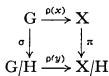
\includegraphics[keepaspectratio]{images/part002_b1d03d5a.jpg}}

Then \(\pi \circ \rho (x) = \rho (y)\circ \sigma\) and hence

\[
\mathrm{T} _ {x} (\pi) \circ \mathrm{T} _ {e} (\rho (x)) = \mathrm{T} _ {e} (\rho (y)) \circ \mathrm{T} _ {e} (\sigma).
\]

Let \(u \in T_{e}(\mathrm{G/H})\) be such that \(T_{e}(\rho(y))u = 0\) . There exists \(v \in T_{e}(\mathrm{G})\) such that \(u = T_{e}(\sigma)v\) . Then \(T_{x}(\pi)(T_{e}(\rho(x))v) = 0\) , hence \(T_{e}(\rho(x))v\) is tangent to Hx (Differentiable and Analytic Manifolds, R, 5.10.5) and therefore is of the form \(T_{e}(\rho(x) | H)v'\) for some \(v' \in T_{e}(\mathrm{H})\) . As \(T_{e}(\rho(x))\) is injective, it follows that \(v = v'\) , whence \(v \in T_{e}(\mathrm{H})\) and therefore \(u = 0\) . Thus \(T_{e}(\rho(y))\) is injective. The image of \(T_{e}(\rho(y))\) is equal to that of \(T_{x}(\pi) \circ T_{e}(\rho(x))\) ; now the image of \(T_{e}(\rho(x))\) admits a topological supplement in \(T_{x}(\mathrm{X})\) and contains the kernel of \(T_{x}(\pi)\) . It is therefore seen that \(\rho(y)\) is an immersion, which completes the proof of (ii).

Assertion (iii) follows from the above and Differentiable and Analytic Manifolds, R, 5.9.7.

COROLLARY. Let G be a Lie group and H and L normal Lie subgroups of G with \(L \subset H\) . Then H/L is a normal Lie subgroup of G/L and the canonical bijection of G/H onto \((G/L)/(H/L)\) is a Lie group isomorphism.

\subsection{ORBITS}

PROPOSITION 14. Let \(\mathbf{G}\) be a Lie group, \(\mathbf{X}\) an analytic manifold and \((g,x)\mapsto gx\) a law of analytic left operation of \(\mathbf{G}\) on \(\mathbf{X}\) . Let \(x\in \mathbf{X}\) . Suppose that the corresponding orbital mapping \(\rho (x)\) is a subimmersion (which is always the case if \(\mathbf{K}\) is of characteristic 0 and \(\mathbf{X}\) is finite-dimensional (Corollary to Proposition 9)). Let \(\mathbf{G}_{\mathbf{x}}\) be the stabilizer of \(x\) in \(\mathbf{G}\) .

\begin{enumerate}
\def\labelenumi{(\roman{enumi})}
\item
  \(\mathrm{G}_x\) is a Lie subgroup and \(\mathrm{T}_e(\mathrm{G}_x) = \mathrm{Ker}\, \mathrm{T}_e(\rho(x))\) .
\item
  The canonical mapping \(i_x\) of the homogeneous space \(G / G_x\) into \(X\) is an immersion with image \(Gx\) .
\item
  If further the orbit \(\mathbf{G}x\) is locally closed and the topology on \(\mathbf{G}\) admits a countable base, then \(\mathbf{G}x\) is a submanifold of \(\mathbf{X}\) , \(i_x\) is an isomorphism of the manifold \(\mathrm{G} / \mathrm{G}_x\) onto the manifold \(\mathbf{G}x\) and \(\mathrm{T}_x(\mathbf{G}x) = \operatorname{Im} \mathrm{T}_e(\rho(x))\) .
\end{enumerate}

The inverse image of \(x\) under \(\rho(x)\) is \(G_x\) . As \(\rho(x)\) is a subimmersion, \(G_x\) is a submanifold and, for all \(g \in G\) , the tangent space \(J\) to \(gG_x = \rho(x)^{-1}(gx)\) at \(g\) is \(\operatorname{Ker} T_g(\rho(x))\) (Differentiable and Analytic Manifolds, R, 5.10.5), whence (i). Let \(\pi: G \to G/G_x\) be the canonical mapping. Then \(i_x \circ \pi = \rho(x)\) . As \(G/G_x\) is a quotient manifold of \(G\) , this equality proves that \(i_x\) is analytic. Further, the kernels of \(T_g(\rho(x))\) and \(T_g(\pi)\) are both equal to \(J\) . Hence \(T_{\pi(g)}(i_x)\) is injective. The image of \(T_{\pi(g)}(i_x)\) is equal to the image of \(T_g(\rho(x))\) and hence admits a topological supplement. This proves (ii).

Suppose that \(Gx\) is locally closed. Every point of \(Gx\) then has a neighbourhood in \(Gx\) which is homeomorphic to a closed subspace of a complete metric space and hence is a Baire space. Hence \(Gx\) is a Baire space (General Topology, Chapter IX, § 5, Proposition 4). If \(G\) has a countable base, \(i_x\) is therefore a homeomorphism of \(G / G_x\) onto \(Gx\) (General Topology, Chapter IX, § 5). Then by (ii) and Differentiable and Analytic Manifolds, R, 5.8.3, \(i_x\) is an isomorphism of the manifolds \(G / G_x\) onto the manifold \(Gx\) and

\[
\mathrm{T} _ {x} (\mathrm{G} x) = \operatorname{Im} \mathrm{T} _ {\pi (e)} (i _ {x}) = \operatorname{Im} \mathrm{T} _ {e} (\rho (x)).
\]

Remark. Let G be a finite-dimensional Lie group, X a manifold of class \(C^{r}\) and \((g, x) \mapsto gx\) a law of left operation of class \(C^{r}\) of G on X. Then Proposition 14 remains valid. The only point which needs a different proof is the fact that \(G_{x}\) is a Lie subgroup. But if \(r \neq \omega\) , K = R; as clearly \(G_{x}\) is closed, \(G_{x}\) is a Lie subgroup by §8, Theorem 2.

COROLLARY. Let G be a Lie group whose topology admits a countable base and X a

non-empty finite-dimensional analytic manifold with a law of analytic left operation of G on X. Suppose that G operates transitively on X and that K is of characteristic 0. Then X is a Lie homogeneous space for G.

Let \(x \in X\) . The orbit of \(x\) , equal to \(X\) , is closed and we can therefore apply Proposition 14 (iii).

\subsection{VECTOR BUNDLES WITH OPERATORS}

Let G be a Lie group, X a manifold of class \(C^{r}\) and \((g, x) \mapsto gx\) a law of left operation of class \(C^{r}\) of G on X. Let E be a vector bundle of class \(C^{r}\) , with base space X and \(\pi: E \to X\) the projection of E onto X. For all \(x \in X\) , let \(E_{x}\) be the fibre of E at x. Let \((g, u) \mapsto gu\) be a law of left operation of G on E such that \(\pi\) is compatible with the operations of G on X and on E. For all \(g \in G\) and all \(x \in X\) , the restriction to \(E_{x}\) of the mapping \(u \mapsto gu\) is a bijection \(\psi_{g,x}\) of \(E_{x}\) onto \(E_{gx}\) . We shall assume that, for all \(g \in G\) and all \(x \in X\) , \(\psi_{g,x}\) is continuous and linear and hence is an isomorphism of the normable space \(E_{x}\) onto the normable space \(E_{gx}\) .

Let \(\phi\) be the automorphism \((g,x)\mapsto (g,gx)\) of the manifold \(\mathrm{G}\times \mathrm{X}\) . Let \(p\) be the canonical projection of \(\mathrm{G}\times \mathrm{X}\) onto \(\mathbf{X}\) and \(\mathrm{E}'\) the inverse image of \(\mathrm{E}\) under \(p\) . Let \(\psi \colon \mathrm{E}'\to \mathrm{E}'\) be the mapping the sum of the \(\psi_{g,x}\colon \mathrm{E}_{(g,x)}'\to \mathrm{E}_{(g,gx)}'\) .

DEFINITION 4. If \(\psi\) is a \(\phi\) -morphism of vector bundles of class \(\mathbf{C}^r\) , \(\mathbf{E}\) is called a vector \(\mathbf{G}\) -bundle of class \(\mathbf{C}^r\) .

In other words, E is a vector G-bundle of class \(C^{r}\) if for all \((g_{0}, x_{0}) \in \mathbf{G} \times \mathbf{X}\) the following condition holds: there exists an open neighbourhood U of \((g_{0}, x_{0})\) in \(G \times X\) such that, if \(E^{\prime} \mid U\) (resp. \(E^{\prime} \mid \phi(U)\) ) is identified with a trivial vector bundle of fibre M (resp. N) by means of a vector chart, the mapping \((g, x) \mapsto \psi_{g,x}\) of U into \(\mathcal{L}(M, N)\) is of class \(C^{r}\) .

The mapping \(\psi\) is obviously bijective and it follows from the above local criterion that \(\psi^{-1}\) is a \(\phi^{-1}\) -morphism of vector bundles so that \(\psi\) is a \(\phi\) -isomorphism of vector bundles.

A trivial vector G-bundle of base X is a vector bundle \(X \times F\) (where F is a complete normable space) with the law of operation \((g, (x, f)) \mapsto (gx, f)\) of G on \(X \times F\) .

We again assume the hypotheses and notation preceding Definition 4 and further take \(\tau\) to be a vector functor of class \(C^r\) for isomorphisms (Differentiable and Analytic Manifolds, R, 7.6.6). Then \(\tau E\) is a vector bundle with base space \(X\) . For all \(x \in X\) , its fibre \((\tau E)_x\) is equal to \(\tau (E_x)\) . For all normable spaces \(N_1, N_2\) , let \(\operatorname{Isom}(N_1, N_2)\) denote the set of isomorphisms of \(N_1\) onto \(N_2\) . If \(g \in G\) , then

\[
\tau (\psi_ {g, x}) \in \operatorname{Isom} ((\tau E) _ {x}, (\tau E) _ {g x}).
\]

The \(\tau(\psi_{g,x})\) define a law of left operation \((g,u)\mapsto gu\) of G on \(\tau\) E and the canonical projection of \(\tau\) E onto X is compatible with the operations of G on X and \(\tau\) E.

PROPOSITION 15. If E is a vector G-bundle of class \(\mathbf{C}^r\) , \(\tau \mathbf{E}\) is a vector G-bundle of class \(\mathbf{C}^r\) .

Let \(g_0, x_0\) , U, M, N be as in the paragraph following Definition 4. Then the mapping \((g, x) \mapsto \tau(\psi_{g,x})\) of U into \(\mathcal{L}(\tau\mathrm{M}, \tau\mathrm{N})\) is the composition of the mapping \((g, x) \mapsto \psi_{g,x}\) of U into \(\mathcal{L}(\mathrm{M}, \mathrm{N})\) and the mapping \(f \mapsto \tau(f)\) of \(\operatorname{Isom}(\mathrm{M}, \mathrm{N})\) into \(\operatorname{Isom}(\tau\mathrm{M}, \tau\mathrm{N})\) ; these two mappings are of class \(C^r\) and hence so is their composition, whence the proposition.

PROPOSITION 16. Let G be a Lie group, X a manifold of class \(\mathbf{C}^r\) ( \(r \geqslant 2\) ) and \((g, x) \mapsto gx\) a law of left operation of class \(\mathbf{C}^r\) of G on X, whence, by transporting the structure, there is a law of left operation of G on TX. Under this law, TX is a vector G-bundle of class \(\mathbf{C}^{r-1}\) .

Let \(\mathrm{pr}_1\) (resp. \(\mathrm{pr}_2\) ) be the canonical projection of \(\mathrm{G} \times \mathrm{X}\) onto \(\mathrm{G}\) (resp. \(\mathrm{X}\) ) and let \(\mathrm{E}_1\) (resp. \(\mathrm{E}_2\) ) be the inverse image of TG (resp. TX) relative to \(\mathrm{pr}_1\) (resp. \(\mathrm{pr}_2\) ). Then the vector bundle \(\mathrm{T}(\mathrm{G} \times \mathrm{X})\) is the direct sum of \(\mathrm{E}_1\) and \(\mathrm{E}_2\) . Let \(i: \mathrm{E}_2 \to \mathrm{T}(\mathrm{G} \times \mathrm{X})\) and \(q: \mathrm{T}(\mathrm{G} \times \mathrm{X}) \to \mathrm{E}_2\) be the canonical vector bundle morphisms defined by this decomposition into a direct sum. Let \(\phi\) be the mapping \((g, x) \mapsto (g, gx)\) of \(\mathrm{G} \times \mathrm{X}\) into \(\mathrm{G} \times \mathrm{X}\) . Then the mapping denoted by \(\psi\) in Definition 4 (where we put \(\mathrm{E} = \mathrm{TX}\) ) is just \(q \circ \mathrm{T}(\phi) \circ i\) . But \(\mathrm{T}(\phi)\) is a \(\phi\) -morphism of vector bundles of class \(\mathrm{C}^{r-1}\) (Differentiable and Analytic Manifolds, R, 8.1.2).

COROLLARY. If \(\tau\) is a vector functor of class \(\mathbf{C}^r\) for isomorphisms, \(\tau(\mathrm{TX})\) is a vector G-bundle of class \(\mathbf{C}^{r-1}\) .

This follows from Propositions 15 and 16.

Remark 1. If \(\tau\) is a vector functor of class \(C^r\) for isomorphisms in finite dimension and \(E\) is of finite rank, \(\tau E\) is defined similarly and Proposition 15 remains valid; the Corollary to Proposition 16 remains valid provided \(X\) is finite-dimensional.

Examples. With the hypotheses and notation of Proposition 16, let F be a complete normable space. Then \(\mathcal{L}((\mathrm{TX})^p; \mathrm{F})\) is a vector G-bundle of class \(\mathrm{C}^{r-1}\) ; so is \(\operatorname{Alt}^p(\mathrm{TX}; \mathrm{F})\) if K is of characteristic zero or X is finite-dimensional (cf.~Differentiable and Analytic Manifolds, R, 7.7, 7.8). If X is finite-dimensional, \(\bigotimes^p(\mathrm{TX}) \otimes \bigotimes^q(\mathrm{TX})^*\) is a vector G-bundle of class \(\mathrm{C}^{r-1}\) .

PROPOSITION 17. Let G be a Lie group, X a left Lie homogeneous space of G, \(x_0\) a point of X, \(G_0\) the stabilizer \(x_0\) in G, E and E' left vector G-bundles of class \(C^{r}\) and base space X, \(E_0\) (resp. \(E_0'\) ) the fibre of E (resp. E') at \(x_0\) and f an element of \(\mathcal{L}(E_0, E_0')\) such that \(f(gu) = g(f(u))\) for all \(u \in E_0\) and \(g \in G_0\) . Then there exists one and only one morphism of E into E' compatible with the operations of G and extending f. The uniqueness of this morphism is obvious. We prove its existence. Let \(g\) , \(g'\) elements of G and \(u \in E_0\) be such that \(gu = g'u\) . Then \(g'^{-1}g \in G_0\) and \(g'^{-1}gu = u\) and hence \(g'^{-1}gf(u) = f(u)\) , that is \(gf(u) = g'f(u)\) . Hence a mapping \(\phi\) is defined of E into \(E'\) by writing \(\phi(gu) = gf(u)\) . Clearly this mapping extends \(f\) and it is compatible with the operations of G. We show that \(\phi\) is a vector bundle morphism of class \(C^r\) . Let \(x_1 \in X\) . There exists an open neighbourhood V of \(x_1\) in X and a submanifold W of G such that the mapping \(g \mapsto gx_0\) is an isomorphism \(\theta\) of class \(C^r\) of W onto V. By shrinking V and W it can be assumed that:

\begin{enumerate}
\def\labelenumi{(\arabic{enumi})}
\item
  E \textbar{} V (resp. E' \textbar{} V) is identified with a trivial vector bundle of fibre M (resp. M');
\item
  if \(\psi_{g}\) (resp. \(\psi_{g}^{\prime}\) ) denotes the mapping \(u\mapsto gu\) of \(\mathrm{E}_0\) (resp. \(\mathrm{E}_0^{\prime}\) ) into \(\mathrm{E}_{gx_0}\) (resp. \(\mathrm{E}_{gx_0}\) ), then the mappings \(g\mapsto \psi_g\) and \(g\mapsto \psi_g^{-1}\) (resp. \(g\mapsto \psi_g^{\prime}\) and \(g\mapsto \psi_g^{\prime -1}\) ) of W into \(\mathcal{L}(\mathrm{E}_0,\mathrm{M})\) and \(\mathcal{L}(\mathrm{M},\mathrm{E}_0)\) (resp. \(\mathcal{L}(\mathrm{E}_0',\mathrm{M}')\) and \(\mathcal{L}(\mathrm{M}',\mathrm{E}_0'))\) are of class \(C^r\) .
\end{enumerate}

For \(x \in V\) , let \(\phi_x: M \to M'\) be the restriction of \(\phi\) to \(E_x = M\) . Then \(\phi_x\) is obtained by composing the following mappings:

\begin{enumerate}
\def\labelenumi{(\arabic{enumi})}
\item
  the mapping \((\psi_{\theta^{-1}(x)})^{-1}\) of M into \(E_{0}\) ;
\item
  the mapping f of \(E_{0}\) into \(E_{0}'\) ;
\item
  the mapping \(\psi_{\theta^{-1}(x)}^{\prime}\) of \(\mathbf{E}_0'\) into \(\mathbf{M}'\) .
\end{enumerate}

Hence we see that the mapping \(x \mapsto \phi_x\) of V into \(\mathcal{L}(\mathbf{M}, \mathbf{M}')\) is of class \(\mathbf{C}^r\) .

COROLLARY 1. Let \(\mathrm{E}_0^{\mathbb{G}_0}\) be the set of elements of \(\mathrm{E}_0\) which are invariant under \(\mathbf{G}_0\) . For all \(u \in \mathrm{E}_0^{\mathbb{G}_0}\) , let \(\sigma_u\) be the mapping of X into E defined by \(\sigma_u(gx_0) = gu\) for all \(g \in G\) .

\begin{enumerate}
\def\labelenumi{(\roman{enumi})}
\item
  The G-invariant sections† of E are of class \(\mathbf{C}^r\) .
\item
  \(u \mapsto \sigma_u\) is a bijection of \(\mathrm{E}_0^{\mathrm{G}_0}\) onto the set of G-invariant sections of E.
\end{enumerate}

Assertion (ii) is obvious. To prove (i) it is sufficient to prove that each section \(\sigma_{u}\) is of class \(C^r\) . Let E' be the trivial G-bundle of base X and fibre \(\mathrm{E}_0^{\mathrm{G}_0}\) . Let \(f\) be the canonical injection of \(\mathrm{E}_0^{\mathrm{G}_0}\) into \(\mathrm{E}_0\) . By Proposition 17 there exists a morphism \(\phi\) of E' into E compatible with the operations of G and extending \(f\) . If \(u \in \mathrm{E}_0^{\mathrm{G}_0}\) and \(g \in \mathrm{G}\) , then

\[
\sigma_ {u} (g x _ {0}) = g u = g f (u) = \phi (g u) = \phi ((u, g x _ {0}))
\]

and hence \(\sigma_u(x) = \phi((u, x))\) for all \(x \in \mathbf{X}\) , which proves our assertion.

*For example, let G be a finite-dimensional real Lie group, \(G_{0}\) a compact Lie subgroup of G and X the homogeneous space \(G/G_{0}\) . Let \(x_{0}\) denote the canonical image of e in X. There exists a positive definite symmetric bilinear form on \(T_{x_{0}}(X)\) invariant under \(G_{0}\) (Integration, Chapter VII, § 3, Proposition 1). Applying the above to \((\mathrm{TX})^{*}\otimes(\mathrm{TX})^{*}\) , we see that there exists on X an analytic Riemannian metric invariant under \(G_{0}\) .

COROLLARY 2. Suppose that \(G_{0}\) operates trivially on \(E_{0}\) . Let \(E'\) be the trivial G-bundle with base space X and fibre \(E_{0}\) . There exists one and only one isomorphism of E onto \(E'\) compatible with the operations of G and extending \(Id_{E_{0}}\) .

This follows immediately from Proposition 17.

Remark 2. In this no., the laws of left operation can be replaced throughout by laws of right operation.

\subsection{LOCAL DEFINITION OF A LIE GROUP}

PROPOSITION 18. Let \(\mathbf{G}\) be a group and \(\mathbf{U}\) and \(\mathbf{V}\) two subsets of \(\mathbf{G}\) containing \(e\) . Suppose that \(\mathbf{U}\) has an analytic manifold structure satisfying the following conditions:

\begin{enumerate}
\def\labelenumi{(\roman{enumi})}
\item
  \(\mathrm{V} = \mathrm{V}^{-1},\mathrm{V}^2\subset \mathrm{U},\mathrm{V}\) is open in U;
\item
  the mapping \((x,y)\mapsto xy^{-1}\) of \(\mathbf{V}\times \mathbf{V}\) into \(\mathbf{U}\) is analytic;
\item
  for all \(g \in \mathbf{G}\) , there exists an open neighbourhood \(\mathbf{V}'\) of \(e\) in \(\mathbf{V}\) such that \(g\mathbf{V}'g^{-1} \subset \mathbf{U}\) and such that the mapping \(x \mapsto gxg^{-1}\) of \(\mathbf{V}'\) into \(\mathbf{U}\) is analytic.
\end{enumerate}

Then there exists one and only one analytic manifold structure on \(\mathbf{G}\) with the following properties:

(α) G with this structure is a Lie group;

(β) V is open in G;

\begin{enumerate}
\def\labelenumi{(\Alph{enumi})}
\setcounter{enumi}{24}
\tightlist
\item
  the manifold structures on G and U induce the same structure on V.
\end{enumerate}

\begin{enumerate}
\def\labelenumi{(\alph{enumi})}
\item
  Let A be an open subset of V and \(v_{0}\) an element of V such that \(v_{0}A \subset V\) . Then \(v_{0}A\) is the set of \(v \in V\) such that \(v_{0}^{-1}v \in A\) and hence is an open subset of V (taking account of (ii)). Moreover, (ii) implies that the mappings \(v \mapsto v_{0}v\) of A onto \(v_{0}A\) and \(v \mapsto v_{0}^{-1}v\) of \(v_{0}A\) onto A are inverse analytic bijections and hence analytic isomorphisms.
\item
  We choose an open neighbourhood \(W\) of \(e\) in \(V\) such that \(W = W^{-1}\) , \(W^3 \subset V\) and there exists a chart \((W, \phi, E)\) of the manifold \(U\) with domain \(W\) . For all \(g \in G\) , let \(\phi_g\) be the mapping \(h \mapsto \phi(g^{-1}h)\) of \(gW\) into \(E\) . We show that the charts \(\phi_g\) of \(G\) are analytically compatible. Let \(g_1, g_2\) be elements of \(G\) such that \(g_1W \cap g_2W \neq \emptyset\) , so that \(g_2^{-1}g_1\) and \(g_1^{-1}g_2\) belong to \(W^2\) . By (a), \(W \cap g_1^{-1}g_2W\) is an open subset of \(W\) and hence
\end{enumerate}

\[
\phi_ {g _ {1}} (g _ {1} \mathrm{W} \cap g _ {2} \mathrm{W}) = \phi (\mathrm{W} \cap g _ {1} ^ {- 1} g _ {2} \mathrm{W})
\]

is an open subset D of E. For \(d \in \mathbf{D}\) ,

\[
\left(\phi_ {g _ {2}} \circ \phi_ {g _ {1}} ^ {- 1}\right) (d) = \phi \left(g _ {2} ^ {- 1} g _ {1} \phi^ {- 1} (d)\right);
\]

by (a) we see that \(\phi_{g_2} \circ \phi_{g_1}^{-1}\) is analytic.

\begin{enumerate}
\def\labelenumi{(\alph{enumi})}
\setcounter{enumi}{2}
\item
  By (b) there exists on \(\mathbf{G}\) an analytic manifold structure such that \((\phi_g)_{g\in G}\) is an atlas on \(\mathbf{G}\) . For all \(g_0\in \mathbf{G}\) , the mapping \(g\mapsto g_0g\) ( \(g\in \mathbf{G}\) ) leaves this atlas invariant and hence is an automorphism of \(\mathbf{G}\) with this manifold structure. In particular condition \((\mathrm{GL}_1)\) is satisfied.
\item
  Let \(v_{0} \in V\) . By (ii) there exists an open neighbourhood \(A\) of \(e\) in \(W\) such that \(v_{0}A \subset V\) . This proves first that \(V\) is open in \(G\) . By (a) the mapping \(v \mapsto v_{0}v\) of \(A\) onto \(v_{0}A\) is an analytic isomorphism with the structures induced by U. By (c) we see that the manifold structures on G and U induce the same structure on \(v_{0}\mathbf{A}\) and hence finally on V.
\item
  by (d), (ii) and (iii), we see that conditions \((\mathrm{GL}_2)\) and \((\mathrm{GL}_3)\) hold. Hence G is a Lie group.
\item
  If a manifold structure on G is compatible with the group structure of G and is such that V is an open submanifold of G, then \((\phi_{g})_{g\in G}\) is an atlas on G. Hence the uniqueness assertion of the proposition.
\end{enumerate}

PROPOSITION 19. Let G be a topological group, H a Lie group and f a homomorphism of the group G into the group H. Suppose that there exist an open neighbourhood of \(e_{G}\) in G, a chart (V, \(\phi\) , E) of the manifold H at \(e_{H}\) and a closed vector subspace F of E admitting a topological supplement, such that \(f(\mathrm{U}) \subset \mathrm{V}\) and \((\phi \circ f)\mid_U\) is a homeomorphism of U onto \(\phi(\mathrm{V}) \cap \mathrm{F}\) . Then there exists a unique manifold structure on G such that f is an immersion; this structure is the inverse image under f of the manifold structure on H. With this structure G is a Lie group.

As translations of G (resp. H) are homeomorphisms (resp. analytic isomorphisms), f satisfies condition (R) of Differentiable and Analytic Manifolds, R, 5.8.1. The first two assertions of the proposition then follow from Differentiable and Analytic Manifolds, R, loc. cit. Consider the commutative diagram

\[
\begin{array}{c} \mathrm{G} \times \mathrm{G} \xrightarrow {m} \mathrm{G} \\ f \times f \Big \downarrow \qquad \qquad \qquad \qquad \qquad \qquad \qquad \qquad \qquad \Big \downarrow f \\ \mathrm{H} \times \mathrm{H} \xrightarrow {n} \mathrm{H} \end{array}
\]

where \(m(x,y)=xy^{-1}\) (resp. \(n(x,y)=xy^{-1}\) ) for x, y in G (resp. H). Then \(n\circ(f\times f)\) is analytic, hence \(f\circ m\) is analytic and hence m is analytic since f is an immersion. Therefore G is a Lie group.

The Lie group structure on G is called the inverse image of the Lie group structure on H under f.

COROLLARY. Let G be a topological group, N a discrete normal subgroup of G and \(\pi\) the canonical mapping of G onto G/N. Suppose that an analytic manifold structure is given on G/N, compatible with the topological group structure on G/N. Then there exists a unique manifold structure on G such that \(\pi\) is an immersion; this structure is the inverse image under \(\pi\) of the manifold structure on G/N. With this structure, \(\pi\) is étale, G is a Lie group and G/N is the quotient Lie group of G by N.

Remark. Let H be a connected real or complex Lie group, \(\hat{H}\) its universal covering \(\dagger\) and \(\pi\) the canonical mapping of \(\hat{H}\) onto H. When we speak of \(\hat{H}\) as a Lie group, we shall always mean with the inverse image structure of that on \(\mathbf{H}\) under \(\pi\) .

\subsection{GROUP GERMS}

DEFINITION 5. A Lie group germ over K is a system (G, e, θ, m) satisfying the following conditions:

\begin{enumerate}
\def\labelenumi{(\roman{enumi})}
\item
  G is an analytic manifold over K;
\item
  \(e \in G;\)
\item
  \(\theta\) is an analytic mapping of G into G;
\item
  \(m\) is an analytic mapping of an open subset \(\Omega\) of \(\mathbf{G} \times \mathbf{G}\) into \(\mathbf{G}\) ;
\item
  for all \(g \in G\) , \((e, g) \in \Omega\) , \((g, e) \in \Omega\) , \(m(e, g) = m(g, e) = g\) ;
\end{enumerate}

\[
g \in G, (g, \theta (g)) \in \Omega , (\theta (g), g) \in \Omega , m (g, \theta (g)) = m (\theta (g), g) = e;
\]

\begin{enumerate}
\def\labelenumi{(\roman{enumi})}
\setcounter{enumi}{6}
\tightlist
\item
  if \(g, h, k\) are elements of \(G\) such that \((g, h) \in \Omega\) , \((h, k) \in \Omega\) , \((m(g, h), k) \in \Omega\) , \((g, m(h, k)) \in \Omega\) , then \(m(m(g, h), k) = m(g, m(h, k))\) .
\end{enumerate}

e is called the identity element of the group germ. We often write gh instead of \(m(g, h)\) and (by an abuse of notation) \(g^{-1}\) instead of \(\theta(g)\) .

A Lie group G is a Lie group germ with the obvious choice of \(e, \theta, m\) . Let G be a Lie group germ. Then \(ee^{-1} = e\) , that is

\[
e ^ {- 1} = e.\tag{8}
\]

For all \(g\in G\)

\[
g = e g = ((g ^ {- 1}) ^ {- 1} g ^ {- 1}) g = (g ^ {- 1}) ^ {- 1} (g ^ {- 1} g) = (g ^ {- 1}) ^ {- 1} e,
\]

that is

\[
(g ^ {- 1}) ^ {- 1} = g.\tag{9}
\]

A subset of G invariant under the mapping \(g \mapsto g^{-1}\) is called symmetric. The manifold G, with the point e, the mapping \(g \mapsto g^{-1}\) and the mapping \((g, h) \mapsto hg\) is a Lie Group germ G \(^{\nu}\) called the opposite of G.

The Lie group germ G is called commutative if, for all \((g,h)\in \mathbf{G}\times \mathbf{G}\) such that \(gh\) is defined, \(hg\) is defined and equal to \(gh\) .

Let \(G\) be a Lie group germ. The set of \((g, h) \in G \times G\) such that \(gh\) is defined is a neighbourhood of \((e, e)\) . On the other hand, the mappings \((g, h) \mapsto gh\) and \(g \mapsto g^{-1}\) are continuous. Hence \((gh)k = g(hk)\) for \(g, h, k\) sufficiently close to \(e\) . Similarly, \((h^{-1}g^{-1})(gh) = h^{-1}(eh) = h^{-1}h = e\) for \(g, h\) sufficiently close to \(e\) , whence multiplying on the right by \((gh)^{-1}\) ,

\begin{enumerate}
\def\labelenumi{(\arabic{enumi})}
\setcounter{enumi}{9}
\tightlist
\item
\end{enumerate}

\((gh)^{-1} = h^{-1}g^{-1}\) for \(g,h\) sufficiently close to \(e\) .

PROPOSITION 20. Let G be a Lie group germ and \(g \in G\) . There exist an open neighbourhood U of e and an open neighbourhood V of g with the following properties:

\begin{enumerate}
\def\labelenumi{(\alph{enumi})}
\item
  ug is defined for all \(u \in U\) ;
\item
  \(vg^{-1}\) is defined for all \(v \in V\) ;
\item
  the mappings \(u \mapsto ug\) , \(v \mapsto vg^{-1}\) are inverse analytic isomorphisms of one another of U onto V and of V onto U.
\end{enumerate}

As the set of definition of the product is open in \(\mathbf{G} \times \mathbf{G}\) , there exist an open neighbourhood U of \(e\) and an open neighbourhood V of \(g\) with properties (a) and (b). Let \(\eta(u) = ug\) for \(u \in \mathrm{U}\) , \(\eta'(v) = vg^{-1}\) for \(v \in \mathrm{V}\) . By shrinking U and V, it can be assumed that \((ug)g^{-1} = u\) and \((vg^{-1})g = v\) for \(u \in \mathrm{U}\) and \(v \in \mathrm{V}\) . Then \(\eta\) and \(\eta'\) are injections. By shrinking U further, it can be assumed that \(\eta(\mathrm{U}) \subset \mathrm{V}\) . Then \(\eta'(\mathrm{V}) \supset \mathrm{U}\) and \(\eta(\mathrm{U})\) is the inverse image of U under \(\eta'\) and hence is an open neighbourhood of \(g\) in V. Replacing V by \(\eta(\mathrm{U})\) , we finally arrive at the situation where \(\eta\) and \(\eta'\) are analytic inverse bijections.

Let \(G_{1}, G_{2}\) be two Lie group germs with identity elements \(e_{1}, e_{2}\) . A mapping f of \(G_{1}\) into \(G_{2}\) is called a morphism if f satisfies the following conditions:

\begin{enumerate}
\def\labelenumi{(\roman{enumi})}
\item
  \(f\) is analytic;
\item
  \(f(e_{1}) = e_{2};\)
\item
  if \(g, h\) are elements of \(\mathbf{G}_1\) such that \(gh\) is defined, then \(f(g)f(h)\) is defined and is equal to \(f(gh)\) .
\end{enumerate}

Let \(g \in G_1\) . As \(gg^{-1}\) is defined and is equal to \(e_1, f(g)f(g^{-1})\) is defined and is equal to \(e_2\) and hence

\[
f (g) ^ {- 1} = f (g) ^ {- 1} \left(f (g) f \left(g ^ {- 1}\right)\right) = \left(f (g) ^ {- 1} f (g)\right) f \left(g ^ {- 1}\right)
\]

that is

\[
f (g) ^ {- 1} = f (g ^ {- 1}).\tag{11}
\]

The composition of two morphisms is a morphism.

If \(f: \mathbf{G}_1 \to \mathbf{G}_2\) and \(f': \mathbf{G}_2 \to \mathbf{G}_1\) are two inverse morphisms of one another, they are isomorphisms (using in particular formula (11)).

Let \(G_{1}\) , \(G_{2}\) be two Lie group germs, and f a mapping of \(G_{1}\) into \(G_{2}\) satisfying conditions (ii) and (iii) above, which is analytic in an open neighbourhood of \(e_{1}\) . Using Proposition 20, it can be proved as in Proposition 4 that f is a morphism.

Let \((\mathbf{G}, e, \theta, m)\) be a Lie group germ and \(\Omega\) the set of definition of \(m\) . Let \(\mathbf{H}\) be a submanifold of \(\mathbf{G}\) containing \(e\) , which is stable under \(\theta\) . Suppose that the set \(\Omega_1\) of \((x, y) \in \Omega \cap (\mathbf{H} \times \mathbf{H})\) such that \(m(x, y) \in \mathbf{H}\) is open in \(\mathbf{H} \times \mathbf{H}\) . Then \((\mathbf{H}, e, \theta | \mathbf{H}, m | \Omega_1)\) is a Lie group germ. Such a Lie group germ is called a Lie subgroup germ of \(\mathbf{G}\) . The canonical injection of \(\mathbf{H}\) into \(\mathbf{G}\) is a morphism. If \(f: \mathbf{L} \to \mathbf{G}\) is a morphism of Lie group germs such that \(f(\mathbf{L}) \subset \mathbf{H}\) , then \(f: \mathbf{L} \to \mathbf{H}\) is a morphism of Lie group germs.

Suppose that K is of characteristic 0. If we replace the hypothesis that H is a submanifold of G by the hypothesis that H is a quasi-submanifold of G, the results of the above paragraph remain true (cf.~Differentiable and Analytic Manifolds, R, 5.8.5). H is then called a Lie quasi-subgroup germ of G.

If G is a Lie group germ with identity element e, every symmetric open neighbourhood of e in G is a Lie subgroup germ of G. (This applies in particular when G is a Lie group.) Let H be a Lie subgroup germ of G; if H is a neighbourhood of e in G, then H is open in G by Proposition 20.

The product Lie group germ of a finite number of Lie group germs is defined in an obvious way.

PROPOSITION 21. Let G, H be two Lie group germs and \(\phi\) a morphism of G into H. The following conditions are equivalent:

\begin{enumerate}
\def\labelenumi{(\roman{enumi})}
\item
  \(\phi\) is étale at \(e\) ;
\item
  there exist open Lie subgroup germs G', H' of G, H such that \(\phi|G'\) is an isomorphism of G' onto H'.
\end{enumerate}

The implication \(\langle \mathrm{ii}\rangle \Rightarrow \langle \mathrm{i}\rangle\) is obvious. Suppose that \(\phi\) is étale at \(e\) . There exists an open Lie subgroup germ \(\mathbf{G}_1\) of \(\mathbf{G}\) such that \(\phi (\mathbf{G}_1)\) is open in \(\mathbf{H}\) and \(\phi |\mathbf{G}_1\) is an isomorphism of the manifold \(\mathbf{G}_1\) onto the manifold \(\phi (\mathbf{G}_1)\) . Then there exists an open Lie subgroup germ \(\mathbf{G}'\) of \(\mathbf{G}_1\) such that the product in \(\mathbf{G}\) of two elements of \(\mathbf{G}'\) is always defined and belongs to \(\mathbf{G}_1\) . If \(g, g'\) are elements of \(\mathbf{G}'\) such that \(\mathrm{gg}^{\prime}\in \mathrm{G}'\) , then \(\phi (g)\phi (g') = \phi (gg')\in \phi (\mathbf{G}')\) ; if \(g, g'\) are elements of \(\mathbf{G}'\) such that \(gg^{\prime}\in G_1 - G'\) , then

\[
\phi (g) \phi (g ^ {\prime}) = \phi (g g ^ {\prime}) \in \phi (\mathrm{G} _ {1}) - \phi (\mathrm{G} ^ {\prime}).
\]

Hence \(\phi |G^{\prime}\) is an isomorphism of the Lie group germ \(G^{\prime}\) onto the open Lie subgroup germ \(\phi (G^{\prime})\) of H.

If the conditions of Proposition 21 hold, G and H are called locally isomorphic.

PROPOSITION 22. Let H be a Lie group, U a Lie subgroup germ of H and N the set of \(g \in \mathrm{H}\) such that U and \(g\mathrm{Ug}^{-1}\) have the same germ at \(e\) (General Topology, Chapter I, § 6, no. 10). Then \(N\) is a subgroup of H containing U. There exists one and only one analytic manifold structure on \(\mathbb{N}\) with the following properties:

\begin{enumerate}
\def\labelenumi{(\roman{enumi})}
\item
  N with this structure is a Lie group;
\item
  U is an open submanifold of N;
\item
  the canonical injection of \(\mathbf{N}\) into \(\mathbf{H}\) is an immersion.
\end{enumerate}

Clearly \(\mathbf{N}\) is a subgroup of \(\mathbf{H}\) . If \(g \in \mathbf{U}\) , then \(ge \in \mathbf{U}\) and \(geg^{-1} \in \mathbf{U}\) , hence \(gu \in \mathbf{U}\) and \(gug^{-1} \in \mathbf{U}\) for \(u\) sufficiently close to \(e\) in \(\mathbf{U}\) and hence the germ of \(g\mathrm{U}g^{-1}\) at \(e\) is contained in that of \(\mathbf{U}\) ; exchanging \(g\) and \(g^{-1}\) , we see that the germs of \(g\mathrm{U}g^{-1}\) and \(\mathbf{U}\) at \(e\) are equal. Hence \(\mathbf{U} \subset \mathbf{N}\) .

Let \(\mathbf{V}\) be an open neighbourhood of \(e\) in \(\mathbf{U}\) such that \(\mathrm{V} = \mathrm{V}^{-1}\) , \(\mathrm{V}^2 \subset \mathrm{U}\) . Conditions (i), (ii), (iii) of Proposition 18 of no. 9 (where \(\mathrm{G}\) is replaced by \(\mathrm{N}\) ) are satisfied. Hence there exists an analytic manifold structure on \(\mathbf{N}\) with the following properties: \((\alpha)\) \(\mathbf{N}\) with this structure is a Lie group; \((\beta)\) \(\mathbf{V}\) is open in \(\mathbf{N}\) ; \((\gamma)\) the manifold structures on \(\mathbf{N}\) and \(\mathbf{U}\) induce the same structure on \(\mathbf{V}\) . Since \(\mathbf{V}\) is a submanifold of \(\mathbf{H}\) , the canonical injection of \(\mathbf{N}\) into \(\mathbf{H}\) is an immersion at \(e\) and hence at every point of \(\mathbf{N}\) . Let \(u \in \mathbf{U}\) . There exists an open neighbourhood \(V'\) of e in V such that the mapping \(v \mapsto vu\) is an analytic isomorphism of \(V'\) onto an open neighbourhood of u in U (Proposition 20) and at the same time onto an open neighbourhood of u in N. Hence U is open in N and the identity mapping of U is an isomorphism with the given manifold structure on U and the open submanifold structure on N; in other words, U is an open submanifold of N.

Finally, we consider an analytic manifold structure on N with properties (i) and (ii) of the proposition and let \(N^{*}\) be the Lie group thus obtained. Then the identity mapping of N into \(N^{*}\) is étale at e and hence a Lie group isomorphism. This proves the uniqueness assertion of the proposition.

Let H be a Lie group, U a Lie quasi-subgroup germ of H and N the set of \(g \in H\) such that U and \(gUg^{-1}\) have the same germ at e. If K is of characteristic 0, there exists on G one and only one manifold structure with properties (i) and (ii) of Proposition 22. The proof is the same as for Proposition 22.

COROLLARY. Preserving the notation of Proposition 22, let G be the subgroup of H generated by U. Then G is an open subgroup of N. There exists one and only one Lie group structure on G such that U is an open submanifold of G and the canonical injection of G into H is an immersion.

Remark. Preserving the notation of Proposition 22 and its corollary, suppose that K is of characteristic 0, that H is finite-dimensional and that the topology on U admits a countable base. Even with all these hypotheses it is possible that G is not closed in H (Exercise 3). But, if G is closed, G is a Lie subgroup of H. For the mapping \((g,h)\mapsto gh\) is a law of analytic left operation of G on H. The orbit of e is G. Our assertion then follows from Propositions 2 (iv) and 14 (iii).

\subsection{LAW CHUNKS OF OPERATION}

Let \((G, e, \theta, m)\) be a Lie group germ and X a manifold of class \(C^r\) .

DEFINITION 6. A law chunk of left operation of class \(\mathbf{C}^r\) of \(\mathbf{G}\) on \(\mathbf{X}\) is a mapping \(\psi\) defined on an open subset \(\Omega\) of \(\mathbf{G} \times \mathbf{X}\) containing \(\{e\} \times \mathbf{X}\) , with values in \(\mathbf{X}\) and with the following properties:

\begin{enumerate}
\def\labelenumi{(\roman{enumi})}
\item
  \(\psi\) is of class \(C^{r}\) ;
\item
  for all \(x \in X\) , \(\psi(e, x) = x\) ;
\item
  there exists a neighbourhood \(\Omega_1\) of \(\{e\} \times \{e\} \times \mathbf{X}\) in \(\mathbf{G} \times \mathbf{G} \times \mathbf{X}\) such that, for \((g, g', x) \in \Omega_1\) , the elements of \(m(g, g')\) , \(\psi(m(g, g'), x)\) , \(\psi(g, \psi(g', x))\) are defined and \(\psi(g, \psi(g', x)) = \psi(m(g, g'), x)\) .
\end{enumerate}

Law chunks of right operation of class \(\mathbf{C}^r\) are defined similarly.

We often write \(gx\) instead of \(\psi(g, x)\) .

Let \(G'\) be a Lie subgroup germ of G and \(X'\) a submanifold of X. Suppose that the set \(\Omega'\) of \((g,x)\in \Omega \cap (\mathrm{G}'\times \mathrm{X}')\) such that \(\psi (g,x)\in \mathrm{X}'\) is open in \(\mathrm{G}'\times \mathrm{X}'\) (a condition which is always fulfilled if \(\mathbf{X}'\) is open in \(\mathbf{X}\) ). Then \(\psi |\Omega '\) is a law chunk of left operation of class \(\mathrm{C}^r\) of \(\mathrm{G}'\) on \(\mathrm{X}'\) , which is said to be derived from \(\psi\) by restriction to \(\mathrm{G}'\) and \(\mathrm{X}'\) .

PROPOSITION 23. Let \((\mathbf{G}, e, \theta, m)\) be a Lie group germ, \(\mathbf{X}\) a manifold of class \(\mathbf{C}^r\) , \(x_0\) a point of \(\mathbf{X}\) , \(\Omega\) an open neighbourhood of \((e, x_0)\) in \(\mathbf{G} \times \mathbf{X}\) and \(\psi\) a mapping of \(\Omega\) into \(\mathbf{X}\) with the following properties:

\begin{enumerate}
\def\labelenumi{(\roman{enumi})}
\item
  \(\psi\) is of class \(C^{r}\) ;
\item
  \(\psi(e, x)\) is equal to x for x sufficiently close to \(x_{0}\) ;
\item
  \(\psi(m(g, g'), x) = \psi(g, \psi(g', x))\) for \((g, g', x)\) sufficiently close to \((e, e, x_0)\) .
\end{enumerate}

Then there exist an open neighbourhood \(\mathbf{X}'\) of \(x_0\) in \(\mathbf{X}\) and an open subset \(\Omega'\) of \(\Omega \cap (\mathrm{G} \times \mathrm{X}')\) such that \(\psi|\Omega'\) is a law chunk of left operation of class \(\mathbf{C}^r\) of \(\mathbf{G}\) on \(\mathbf{X}'\) .

There exist an open neighbourhood \(\mathbf{X}'\) of \(x_0\) in \(\mathbf{X}\) and an open neighbourhood \(\mathbf{G}'\) of \(e\) in \(\mathbf{G}\) such that \(\psi(e, x) = x\) for all \(x \in \mathbf{X}'\) , and

\[
\psi (g, \psi (g ^ {\prime}, x)) = \psi (m (g, g ^ {\prime}), x)
\]

for \((g, g', x) \in \mathrm{G}' \times \mathrm{G}' \times \mathrm{X}'\) . Let \(\Omega'\) be the set of \((g, x) \in \Omega \cap (\mathrm{G}' \times \mathrm{X}')\) such that \(\psi(g, x) \in \mathrm{X}'\) . Then \(\Omega'\) is open in \(\mathrm{G} \times \mathrm{X}'\) and \(\mathrm{X}'\) , \(\Omega'\) have the properties of the proposition.

Lemma 3. Let \(\mathbf{X}\) be a normal space and \((\mathbf{X}_i)_{i\in I}\) a locally finite open covering of \(\mathbf{X}\) . For all \((i,j)\in I\times I\) and all \(x\in \mathbf{X}_i\cap \mathbf{X}_j\) , let \(\mathrm{V}_{ij}(x)\) be a neighbourhood of \(x\) contained in \(\mathbf{X}_i\cap \mathbf{X}_j\) . Then we can associate with every \(x\in X\) a neighbourhood \(\mathrm{V}(x)\) of \(x\) such that the following conditions are fulfilled:

\begin{enumerate}
\def\labelenumi{(\alph{enumi})}
\item
  the relation \(x \in \mathbf{X}_i \cap \mathbf{X}_j\) implies \(\mathrm{V}(x) \subset \mathrm{V}_{ij}(x)\) ;
\item
  if \(\mathrm{V}(x)\) and \(\mathrm{V}(y)\) meet, there exists \(i\in \mathbf{I}\) such that \(\mathrm{V}(x)\cup \mathrm{V}(y)\subset \mathrm{X}_i\)
\end{enumerate}

There exists an open covering \(\langle \mathrm{X}_i\rangle_{i\in I}\) of \(\mathbf{X}\) such that \(\overline{\mathbf{X}}_i' \subset \mathbf{X}_i\) for all \(i \in I\) (General Topology, Chapter IX, § 4, Theorem 3). Let \(x \in \mathbf{X}\) . Let \(\mathrm{V}_1(x)\) be the intersection of the \(\mathrm{V}_{ij}(x)\) and the \(\mathbf{X}_k'\) which contain \(x\) ; this is an open neighbourhood of \(x\) . Let \(\mathrm{V}_2(x)\) be a neighbourhood of \(x\) contained in \(\mathrm{V}_1(x)\) and meeting only a finite number of \(\mathbf{X}_i\) . Then \(\mathrm{V}_2(x)\) meets only a finite number of \(\overline{\mathbf{X}}_i'\) and hence the set

\[
\mathrm{V} (x) = \mathrm{V} _ {2} (x) \cap \bigcap_ {i \in I, x \notin \overline {{\mathrm{X}}} _ {i} ^ {\prime}} (\mathrm{X} - \overline {{\mathrm{X}}} _ {i} ^ {\prime})
\]

is a neighbourhood of \(x\) . If \(x \in \mathrm{X}_1 \cap \mathrm{X}_j\) , then \(\mathrm{V}_1(x) \subset \mathrm{X}_1 \cap \mathrm{X}_j\) and hence \(\mathrm{V}(x) \subset \mathrm{X}_1 \cap \mathrm{X}_j\) . Let \(x, y\) be in \(\mathrm{X}\) and suppose that \(\mathrm{V}(x)\) and \(\mathrm{V}(y)\) meet. There exists \(i \in I\) such that \(x \in \mathrm{X}_i'\) . Then \(\mathrm{V}_1(x) \subset \mathrm{X}_i'\) , hence \(\mathrm{V}(x) \subset \mathrm{X}_i'\) and hence \(\mathrm{V}(y) \cap \overline{\mathrm{X}_i'} \neq 0\) . Then \(y \in \overline{\mathrm{X}_i'}\) by definition of \(\mathrm{V}(y)\) , whence \(y \in \mathrm{X}_i\) and \(\mathrm{V}(y) \subset \mathrm{X}_i\) . Thus \(\mathrm{X}_i\) contains \(\mathrm{V}(x)\) and \(\mathrm{V}(y)\) .

PROPOSITION 24. Let G be a Lie group germ, X a manifold of class \(C^{r}\) and (X \(_{i}\) ) \(_{i \in I}\) a locally finite open covering of X. For all i ∈ I, let \(\psi_{i}\) be a law chunk of left operation of class \(C^{r}\) of G on X \(_{i}\) . Suppose that the underlying topological space of X is normal and that, for all (i, j) ∈ I × I and all x ∈ X \(_{i}\) ∩ X \(_{j}\) , \(\psi_{i}\) and \(\psi_{j}\) coincide on a neighbourhood of (e, x). There exists a law chunk \(\psi\) of left operation of class \(C^{r}\) of G on X such that, for all i ∈ I and all x ∈ X \(_{i}\) , \(\psi_{i}\) and \(\psi\) coincide on a neighbourhood of (e, x).

For all \((i,j)\in \mathrm{I}\times \mathrm{I}\) and all \(x\in \mathrm{X}_i\cap \mathrm{X}_j\) choose an open neighbourhood \(\mathrm{V}_{ij}(x)\) of \(x\) in \(\mathrm{X}_i\cap \mathrm{X}_j\) such that \(\psi_i\) and \(\psi_j\) are defined and equal on a neighbourhood of \(\{e\} \times \mathrm{V}_{ij}(x)\) in \(\mathrm{G}\times \mathrm{X}\) . For all \(x\in \mathrm{X}\) choose an open neighbourhood \(\mathrm{V}(x)\) of \(x\) in \(\mathrm{X}\) such that conditions (a) and (b) of Lemma 3 are fulfilled. Let \(\mathbf{I}_x\) be the set of \(i\in \mathrm{I}\) such that \(x\in \mathrm{X}_i\) . This is a finite set. Let \(\mathrm{U}_x\) be the set of \((g,y)\in \mathrm{G}\times \mathrm{V}(x)\) such that the \(\psi_i\) for \(i\in \mathrm{I}_x\) are defined and coincide on a neighbourhood of \((g,y)\) . Then \(\mathrm{U}_x\) is open and \((e,x)\in \mathrm{U}_x\) . The \(\psi_i\) for \(i\in \mathrm{I}_x\) all have the same restriction to \(\mathrm{U}_x\) . Let \(x,y\) be in \(\mathrm{X}\) . If \(\mathrm{U}_x\) and \(\mathrm{U}_y\) meet, \(\mathrm{V}(x)\) and \(\mathrm{V}(y)\) meet and hence there exists \(i\in \mathrm{I}\) such that

\[
\mathrm{V} (x) \cup \mathrm{V} (y) \subset \mathrm{X} _ {i}.
\]

Then \(i \in \mathrm{I}_x, i \in \mathrm{I}_y, \psi_i | \mathrm{U}_x = \psi_x, \psi_i | \mathrm{U}_y = \psi_y\) and hence

\[
\psi_ {x} | (\mathrm{U} _ {x} \cap \mathrm{U} _ {y}) = \psi_ {y} | (\mathrm{U} _ {x} \cap \mathrm{U} _ {y}).
\]

The \(\psi_x\) therefore define a mapping \(\psi\) of \(\mathbf{U} = \bigcup_{x\in \mathbf{X}}\mathbf{U}_x\) into \(\mathbf{X}\) and \(\mathbf{U}\) is an open neighbourhood of \(\{e\} \times \mathbf{X}\) in \(\mathbf{G}\times \mathbf{X}\) . Clearly \(\psi\) is of class \(C^r\) and \(\psi (e,x) = x\) for all \(x\in \mathbf{X}\) . For all \(i\in \mathbf{I}\) and all \(x\in \mathrm{X}_i\) , \(\psi\) coincides with \(\psi_x\) and hence with \(\psi_i\) in a neighbourhood of \((e,x)\) and hence \(\psi\) satisfies condition (iii) of Definition 6.

\section{GROUP OF TANGENT VECTORS TO A LIE GROUP}

\subsection{TANGENT LAWS OF COMPOSITION}

Let X and Y be manifolds of class \(C^{r}\) . We know (Differentiable and Analytic Manifolds, R, 8.1.4) that \(X \times Y\) is a manifold of class \(C^{r}\) and that the mapping \((\mathrm{T}(\mathrm{pr}_{1}), \mathrm{T}(\mathrm{pr}_{2}))\) , the product of the tangent mappings to the canonical projections, is an isomorphism of class \(C^{r-1}\) of \(\mathrm{T}(\mathrm{X} \times \mathrm{Y})\) onto \(\mathrm{T}(\mathrm{X}) \times \mathrm{T}(\mathrm{Y})\) . This isomorphism is compatible with the vector bundle structures with base space \(X \times Y\) and allows us to identify \(\mathrm{T}(\mathrm{X} \times \mathrm{Y})\) with \(\mathrm{T}(\mathrm{X}) \times \mathrm{T}(\mathrm{Y})\) . Let \(a \in \mathbf{X}, b \in \mathbf{Y}, u \in \mathrm{T}_a(\mathbf{X}), v \in \mathrm{T}_b(\mathbf{Y})\) ; the above identification allows us to consider \((u, v)\) as an element of \(\mathrm{T}_{(a,b)}(\mathbf{X} \times \mathbf{Y})\) ; then

\[
(u, v) = (u, 0) + (0, v)
\]

and \((u,0)\) (resp. \((0,v))\) is the image of \(u\) (resp. \(v\) ) under the tangent mapping to the immersion \(x\mapsto (x,b)\) (resp. \(y\mapsto (a,y)\) ) of X (resp. Y) into \(\mathbf{X}\times \mathbf{Y}\) . When it is necessary to be precise, we shall write \(0_{a}\) for the zero element of \(\mathrm{T}_a(X)\) .

Now let X, Y, Z be manifolds of class \(C^{r}\) and f a mapping of class \(C^{r}\) of \(X \times Y\) into Z. The tangent mapping is, using the above identification, a mapping of class \(C^{r-1}\) of \(T(X) \times T(Y)\) into \(T(Z)\) . For \(u \in T_{a}(X)\) and \(v \in T_{b}(Y)\) ,

\begin{enumerate}
\def\labelenumi{(\arabic{enumi})}
\tightlist
\item
\end{enumerate}

\[
\mathrm{T} (f) (u, v) = \mathrm{T} (f) (u, 0 _ {b}) + \mathrm{T} (f) (0 _ {a}, v),
\]

\[
\mathrm{T} (f) \left(0 _ {a}, 0 _ {b}\right) = 0 _ {f (a, b)}.\tag{2}
\]

On the other hand, the mapping \(y \mapsto f(a, y)\) is the composition of the immersion \(y \mapsto (a, y)\) and f; it follows that

\begin{enumerate}
\def\labelenumi{(\arabic{enumi})}
\setcounter{enumi}{2}
\item
  \(\mathrm{T}(f)(0,v)\) is the image of v under the tangent mapping to \(y\mapsto f(a,y)\) . Similarly
\item
  \(\mathbf{T}(f)(u,0)\) is the image of \(u\) under the tangent mapping to \(x\mapsto f(x,b)\) .
\end{enumerate}

If the mapping \(f\) of \(\mathbf{X} \times \mathbf{Y}\) into \(\mathbf{Z}\) is denoted by \((x, y) \mapsto xy\) , \(uv\) is often used to denote the element \(T(f)(u, v)\) for \(u \in T(\mathbf{X})\) , \(v \in T(\mathbf{Y})\) .

Let X be a manifold of class \(C^{r}\) and \(m: X \times X \to X\) a law of composition of class \(C^{r}\) on X. Then \(T(m)\) is a law of composition of class \(C^{r-1}\) on \(T(X)\) . It is called the law of composition tangent to m. The canonical projection p of \(T(X)\) onto X is compatible with the laws m and \(T(m)\) ; in other words,

\[
p \circ \mathrm{T} (m) = m \circ (p \times p).\tag{5}
\]

It follows from (2) that

\[
\mathrm{T} (m) \left(0 _ {x}, 0 _ {y}\right) = 0 _ {m (x, y)}\tag{6}
\]

for all \(x, y\) in \(\mathbf{X}\) ; in other words, the zero section \(x \mapsto 0_x\) of \(\mathrm{T}(\mathbf{X})\) is compatible with the laws \(m\) and \(\mathrm{T}(m)\) .

PROPOSITION 1. Let X be a manifold of class \(\mathbf{C}^r\) and \(m\) a law of composition of class \(\mathbf{C}^r\) on X. If \(m\) is associative (resp. commutative), then \(\mathrm{T}(m)\) is associative (resp. commutative).

If \(m\) is associative, then \(m \circ (m \times \mathrm{Id}_{\mathbf{x}}) = m \circ (\mathrm{Id}_{\mathbf{x}} \times m)\) , whence

\[
\mathrm{T} (m) \circ (\mathrm{T} (m) \times \mathrm{Id} _ {\mathrm{T} (\mathbf {X})}) = \mathrm{T} (m) \circ (\mathrm{Id} _ {\mathrm{T} (\mathbf {X})} \times \mathrm{T} (m))
\]

and hence \(\mathrm{T}(m)\) is associative. Let \(s\) be the mapping \((x,y)\mapsto (y,x)\) of \(\mathbf{X}\times \mathbf{X}\) into \(\mathbf{X}\times \mathbf{X}\) . If \(m\) is commutative, then \(m\circ s = m\) and hence

\[
\mathrm{T} (m) \circ \mathrm{T} (s) = \mathrm{T} (m).
\]

But \(\mathrm{T}(s)\) is the mapping \((u,v)\mapsto (v,u)\) of \(\mathrm{T}(\mathbf{X})\times \mathrm{T}(\mathbf{X})\) into \(\mathrm{T}(\mathbf{X})\times \mathrm{T}(\mathbf{X})\) . Hence \(\mathrm{T}(m)\) is commutative.

PROPOSITION 2. Let X be a manifold of class \(\mathbf{C}^r\) , \(m\) a law of composition of class \(\mathbf{C}^r\) on X and \(e\) an identity element for \(m\) .

\begin{enumerate}
\def\labelenumi{(\roman{enumi})}
\item
  The vector \(0_{e}\) is an identity element for \(\mathbf{T}(m)\) .
\item
  \(\mathrm{T}_{e}(\mathbf{X})\) is stable under \(\mathrm{T}(m)\) and the law of composition induced on \(\mathrm{T}_{e}(\mathbf{X})\) by \(\mathrm{T}(m)\) is the vector space addition on \(\mathrm{T}_{e}(\mathbf{X})\) .
\item
  Let U be an open subset of X and \(\alpha\) a mapping of class \(C^{r}\) of U into X such that, for all \(x \in U\) , \(\alpha(x)\) is the inverse of x under m. Then, for all \(u \in T(U)\) , \(T(\alpha)u\) is the inverse of u under \(T(m)\) .
\end{enumerate}

Properties (3) and (4) show that \(\mathrm{T}(m)(0_e,u) = \mathrm{T}(m)(u,0_e) = u\) for all \(u\in \mathrm{T}(\mathbf{X})\) , whence (i). For \(u,v\) in \(\mathrm{T}_e(\mathbf{X})\) ,

\[
\mathrm{T} (m) (u, v) = \mathrm{T} (m) (u, 0 _ {e}) + \mathrm{T} (m) (0 _ {e}, v) = u + v,
\]

whence (ii). Finally the relations \(m(x, \alpha(x)) = m(\alpha(x), x) = e\) for all \(x \in \mathbf{U}\) imply

\[
\mathrm{T} (m) (u, \mathrm{T} (\alpha) (u)) = \mathrm{T} (m) (\mathrm{T} (\alpha) u, u) = 0 _ {e}
\]

for all \(u \in \mathrm{T}(\mathrm{U})\) , whence (iii).

PROPOSITION 3. Let \(\mathbf{X}_1, \mathbf{X}_2, \ldots, \mathbf{X}_p\) , Y be manifolds of class \(\mathbf{C}^r\) , i an integer of \([1, p]\) , \(m_t\) (resp. n) a law of composition of class \(\mathbf{C}^r\) on \(\mathbf{X}_t\) (resp. Y) and u a mapping of class \(\mathbf{C}^r\) of \(\mathbf{X}_1 \times \mathbf{X}_2 \times \dots \times \mathbf{X}_p\) into Y. If u is distributive relative to the variable of index i, then T(u) is distributive relative to the variable of index i.

The proof is analogous to that of Proposition 1.

\subsection{GROUP OF TANGENT VECTORS TO A LIE GROUP}

PROPOSITION 4. Let G be a Lie group. Then T(G), with the law of composition tangent to the multiplication of G, is a Lie group. The identity element of T(G) is the vector \(0_{e}\) .

This follows from Propositions 1 and 2.

PROPOSITION 5. Let G and H be Lie groups and f a morphism of G into H. Then T(f) is a morphism of the Lie group T(G) into the Lie group T(H).

We know that \(\mathrm{T}(f)\) is analytic. On the other hand, let m (resp. n) denote the multiplication on G (resp. H). Then \(f \circ m = n \circ (f \times f)\) , whence

\[
\mathrm{T} (f) \circ \mathrm{T} (m) = \mathrm{T} (n) \circ (\mathrm{T} (f) \times \mathrm{T} (f)),
\]

which expresses the fact that \(T(f)\) is a group homomorphism.

COROLLARY. Let \(G_{1},\ldots,G_{n}\) be Lie groups. The canonical isomorphism of the manifold \(\mathrm{T}(\mathrm{G}_{1}\times\cdots\times\mathrm{G}_{n})\) onto the manifold \(\mathrm{T}(\mathrm{G}_{1})\times\cdots\times\mathrm{T}(\mathrm{G}_{n})\) is a Lie group isomorphism.

\(pr_{i}\) is a morphism of \(G_{1} \times \cdots \times G_{n}\) into \(G_{i}\) and hence \(T(pr_{i})\) is a morphism of \(T(G_{1} \times \cdots \times G_{n})\) into \(T(G_{i})\) .

PROPOSITION 6. Let G be a Lie group.

\begin{enumerate}
\def\labelenumi{(\roman{enumi})}
\item
  The canonical projection \(p: \mathrm{T}(\mathrm{G}) \to \mathrm{G}\) is a Lie group morphism.
\item
  The kernel of \(p\) is \(\mathrm{T}_e(\mathrm{G})\) . It is a Lie subgroup of \(\mathrm{T}(\mathrm{G})\) . The Lie group structure induced on \(\mathrm{T}_e(\mathrm{G})\) by that on \(\mathrm{T}(\mathrm{G})\) is the Lie group structure of the complete normable space \(\mathrm{T}_e(\mathrm{G})\) .
\item
  The zero section \(s\) is an isomorphism of the Lie group \(\mathbf{G}\) onto a Lie subgroup \(s(\mathbf{G})\) of \(\mathrm{T}(\mathbf{G})\) (which subgroup we identify with \(\mathbf{G}\) ).
\item
  The Lie group T(G) is the semi-direct product of G by \(T_{e}(G)\) .
\end{enumerate}

Assertion (i) follows from (5). Assertion (ii) is obvious taking account of Proposition 2 (ii). Assertions (iii) and (iv) follow from (6) and § 1, Proposition 8.

Let \(u \in \mathrm{T}(\mathrm{G})\) and \(g \in \mathrm{G}\) . By (3) and (4), the products \(ug\) , \(gu\) calculated in the group \(\mathrm{T}(\mathrm{G})\) are the images of \(u\) under \(\mathrm{T}(\delta(g^{-1}))\) and \(\mathrm{T}(\gamma(g))\) . It follows from § 1, Corollary 2 to Proposition 17 that the mapping \((g, u) \mapsto gu\) of \(\mathrm{G} \times \mathrm{T}_e(\mathrm{G})\) into \(\mathrm{T}(\mathrm{G})\) is an isomorphism of the trivial vector bundle \(\mathrm{G} \times \mathrm{T}_e(\mathrm{G})\) with base space \(G\) onto the vector bundle \(\mathrm{T}(\mathrm{G})\) . The inverse isomorphism is called the left trivialization of \(\mathrm{T}(\mathrm{G})\) . By considering the mapping \((g, u) \mapsto ug\) , the right trivialization of \(\mathrm{T}(\mathrm{G})\) is defined similarly.

PROPOSITION 7. Let G be a Lie group, M a manifold of class \(\mathbf{C}^r\) and \(f\) and \(g\) mappings of class \(\mathbf{C}^r\) of M into G, so that \(fg\) is a mapping of class \(\mathbf{C}^r\) of M into G. Let \(m \in \mathbf{M}\) , \(x = f(m)\) , \(y = g(m)\) , \(u \in \mathrm{T}_m(\mathbf{M})\) . Then

\[
(\mathrm{T} f g) u = \mathrm{T} (f) u. y + x. \mathrm{T} (g) u.
\]

Let \(m\) be the multiplication of G. Then \(fg = m \circ (f, g)\) . Now

\[
\mathrm{T} (f, g) (u) = (\mathrm{T} (f) u, \mathrm{T} (g) u),
\]

hence \(\mathrm{T}(fg)u = \mathrm{T}(f)u.\mathrm{T}(g)u\) . It then suffices to apply (1) with \(f\) replaced by \(m\) .

COROLLARY. Let \(n \in \mathbf{Z}\) . The tangent mapping at \(e\) to the mapping \(g \mapsto g^n\) of \(G\) into \(G\) is the mapping \(x \mapsto nx\) of \(T_e(G)\) into \(T_e(G)\) .

For \(n \geqslant 0\) , this follows by induction on \(n\) from Proposition 7. On the other hand, the tangent mapping at \(e\) to the mapping \(g \mapsto g^{-1}\) is the mapping \(x \mapsto -x\) (no. 1, Proposition 2).

Let G be a Lie group, X a manifold of class \(C^r\) and \((g, x) \mapsto gx\) a law of left operation of class \(C^r\) of G on X. Arguing as for Proposition 1, we derive a law of left operation of class \(C^{r-1}\) of T(G) on T(X), which we shall also denote by \((u, v) \mapsto uv\) . Identifying G (resp. X) with the image of the zero section of T(G) (resp. T(X)), we see by (6) that the law of left operation of T(G) on T(X) extends the law of left operation of G on X. For all \(u \in \mathrm{T}_{g}(G)\) and \(v \in \mathrm{T}_{x}(X)\) , by (1),

\[
u v = g v + u x.\tag{7}
\]

If \(g \in G\) and \(v \in T_x(X)\) , \(gv\) is, by (3), the image of \(v\) under the tangent mapping at \(x\) to the mapping \(y \mapsto gy\) of \(X\) into \(X\) . This tangent mapping is an isomorphism of \(T_x(X)\) onto \(T_{gx}(X)\) . In particular,

\[
g (v + v ^ {\prime}) = g v + g v ^ {\prime}, \quad g (\lambda v) = \lambda (g v) \quad \text { for } v, v ^ {\prime} \text { in } T _ {x} (X), \lambda \in K.\tag{8}
\]

If \(x \in \mathbf{X}\) and \(u \in \mathrm{T}_g(\mathrm{G})\) , \(ux\) is by (4) the image of \(u\) under the tangent mapping at \(g\) to the mapping \(h \mapsto hx\) of \(\mathbf{G}\) into \(\mathbf{X}\) . Hence

\[
(9) \quad (u + u ^ {\prime}) x = u x + u ^ {\prime} x, \qquad (\lambda u) x = \lambda (u x) \quad \text { for } u, u ^ {\prime} \text { in } \mathrm{T} _ {g} (\mathrm{G}), \lambda \in \mathrm{K}.
\]

The above can be applied to the case of a Lie group operating on itself by left (resp. right) translation. The corresponding law of operation of T(G) on T(G) is defined by left (resp. right) translation of the Lie group T(G). Formulae (7), (8) and (9) are therefore valid in T(G).

PROPOSITION 8. Let \(\mathbf{G}_1\) and \(\mathbf{G}_2\) be Lie groups, \(\mathbf{X}_1\) and \(\mathbf{X}_2\) manifolds of class \(\mathbf{C}^r\) and \(f_i\) a law of left operation of class \(\mathbf{C}^r\) of \(\mathbf{G}_i\) on \(\mathbf{X}_i\) ( \(i = 1, 2\) ). Let \(\phi\) be a morphism of \(\mathbf{G}_1\) into \(\mathbf{G}_2\) and \(\psi\) a \(\phi\) -morphism of \(\mathbf{X}_1\) into \(\mathbf{X}_2\) . Then \(\mathrm{T}(\psi)\) is a \(\mathrm{T}(\phi)\) -morphism of \(\mathrm{T}(\mathbf{X}_1)\) into \(\mathrm{T}(\mathbf{X}_2)\) .

\(f_{2}\circ (\phi \times \psi) = \psi \circ f_{1},\) whence

\[
\mathrm{T} (f _ {2}) \circ (\mathrm{T} (\phi) \times \mathrm{T} (\psi)) = \mathrm{T} (\psi) \circ \mathrm{T} (f _ {1}).
\]

Let G be a Lie group, X a manifold of class \(C^{r}\) and \((g, x) \mapsto gx\) a law of left operation of class \(C^{r}\) of G on X. Let I be an open subset of K containing 0 and \(\gamma: I \to G\) a mapping of class \(C^{r}\) such that \(\gamma(0) = e\) . Let

\[
a = \mathrm{T} _ {0} (\gamma) 1 \in \mathrm{T} _ {e} (\mathrm{G}).
\]

Let \(x \in X\) . Using (4), \(ax\) is the image under the tangent mapping to \(\lambda \mapsto \gamma(\lambda)x\) of the tangent vector 1 to I at 0. Hence the vector field \(x \mapsto ax\) on \(X\) is the vector field defined by the mapping \((\lambda, x) \mapsto \gamma(\lambda)x\) in the sense of Differentiable and Analytic Manifolds, R, 8.4.5.
